
\documentclass{llncs}
\usepackage{graphicx}        % standard LaTeX graphics tool
                             % when including figure files
\usepackage{subfigure}
\usepackage{url}
%%%%%%%%%%%%%%%%%%%%%%%%%%%%%%%%%%%%%%%%%%%%%%%%%%%%%%%%%%%%%%%%%%%%%%%%%%%%%%%%%%%%%%%%%

\begin{document}
\sloppy

\title{Random Selection of Parameters in Asynchronous Pool-Based Evolutionary Algorithms}

\author{Mario Garc\'ia-Valdez\inst{1} \and Ren\'e M\'arquez\inst{1} \and Juan J. Merelo Guerv\'os\inst{2} \and  Leonardo Trujillo \inst{1}}

\institute{Instituto Tecnol\'ogico de Tijuana, Tijuana BC, Mexico
\and
Universidad de Granada, Granada, Spain
\email{mario@tectijuana.edu.mx}\\
\email{renemarquezvalenzuela@gmail.com}\\
\email{jmerelo@geneura.ugr.es}\\
\email{leonardo.trujillo@tectijuana.edu.mx}}

\maketitle

\begin{abstract}
It is not always possible to set up an distributed system with
homogeneous nodes to run algorithms in a synchronous way. In grid,
cloud or volunteer setups nodes are heterogeneous, or simply are not
available at the exact same time; this is a challenge for the researcher if
their full performance is going to be actually leveraged. We are
interested in evolutionary algorithms (EAs), which evolve a population
of solutions using a mechanism inspired by biological evolution; in this field, 
several asynchronous Evolutionary Algorithms (EAs) that distribute the
evolutionary process among heterogeneous nodes have
been proposed. These algorithms make the population shared between
distributed workers  which execute the actual evolutionary
process by taking samples of the population, and replacing them in the
population pool by evolved individuals. The performance of these EAs
depends in part on the selection of parameters for the EA running in
each worker, which may include sample size, generations, mutation rate
and crossover rate along with the overall configuration. In this paper
we present a method inspired by a strategy proposed by Gong and Fukunaga for the
Island-Model which statically assigns random parameter settings to
each island in a cloud setting. Experiments were conducted in the
cloud using 2, 6 and 12 virtual machine configurations, with
both homogeneous and heterogeneous random settings using five 
test functions for single-objective optimization (Rastrigin, Griewank, De Jong, Schaffer 
and Ackley) and the OneMax binary problem. The results suggest that this approach can yield
performance improvements which are competitive with instances of the
algorithm using workers with control parameters tuned specifically for
the benchmark.

\keywords{Distributed Evolutionary Algorithms, Volunteer Computing,
  Cloud Computing}
\end{abstract}
\section{Introduction}
% EA Paramaters 
% Worst on many workers
% Explore and Exploit
% Dynamic adaptation
% Random Patameters
% Evaluate in EvoSpace

\section{Related Work}
% Dynamic adaptation
% Random Patameters

\section{EvoSpace Cloud Implementation}
% Architecture Components
% Random Patameters
\begin{figure*}[t]
    \centering
        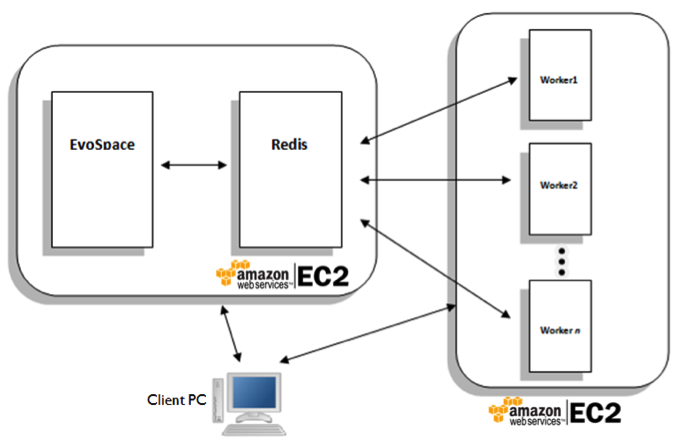
\includegraphics[width=10cm]{img/evospace-aws.png}
    \caption{Main components and data-flow in the cloud version of EvoSpace. }
    \label{fig:evospace}
\end{figure*}

\section{Experimental Set-up}
The goal of this work is to determine if a random static parametrization for each of the $n$ EvoWorkers 
collaborating on a given run could achieve competitive results against an homogeneous tuned parametrization.
The parameters considered to be randomly set for each EvoWorker where the crossover and mutation probabilities 
with a valid range of [0,1]. This parameters where selected because they have a well stablished relationship 
with the exploration and explatation of the solution space \cite{}. Depending on the type of experiment 
and the number of workers the homogeneous values were set for other variables, these are summarized
in Table \ref{tab:params}. Additionally, for all the OneMax experiments a BitFlip mutation was used t
with an independent probability for each attribute to be flipped of 0.05, and a tournament selection of size 3
was used.    


\begin{table}[!t]
\caption{Valid ranges for each EvoWorker parameters. One Max}
\label{tab:params}
\centering
\begin{tabular}{|l|c|c|c|c|c|c| }
\hline
\textbf{Parameter} & \multicolumn{3}{|c|}{OneMax} & \multicolumn{3}{|c|}{Test Functions} \\
\hline
Number of Workers & 2 & 6 & 12 & 2 & 6 & 12\\
\hline
\hline
Population Size & 200 & 280 & 620 & 120 & 150 & 150\\
\hline
Sample Size & 40 & 40 & 40 & 40 & 20 & 10\\
\hline
Maximum Samples & 30 & 40 & 40 & 200 & 100 & 50\\
\hline
Local Generations & 30 & 30 & 30 & 100 & 100 & 100\\
\hline
\end{tabular}
\end{table}

To measure the effectiveness of RPSS in EvoSpace two parametrization strategies are compared, 
similar to what is done in \cite{fuku1,fuku2}. First, we consider the approach of setting all 
of the EvoWorker parameters homogeneously. In order to tune the homogeneous parameters,
we must select the best configuration found after from generating a 100 random parameterizations 
and performing 10 independent runs for each problem. We call this the homogeneous configuration and 
is compared against a random-heterogeneous-parametrization, where the parameters of each worker are 
set independently at random at the beginning of each run; we call this the heterogeneous configuration.
Finally, we perform 30 independent runs of with both methods and report the average number of evaluations.

The algorithms are first evaluated using the OneMax (or BitCounting) problem proposed by 
Schaffer and Eshelman \cite{SE91}, this is a simple problem consisting in maximizing the number 
of ones of a bitstring. For the current experiments a 128 bit string was used. This problem was
selected first because is not computationally demanding, and more experiments where conducted for
the tuning phase, tuning the parameters using 2, 6, and 12 worker configurations. 
Then, following \cite{fuku1}, five standard real-valued single-value optimization problems 
are used, these are the Rastrigin, Griewank, De Jong, Schaffer  and Ackley functions, 
with the number of dimensions set to 100 in each case. For the OneMax problem a standard bitstring 
representation is used, while the other five problems use a real-valued vector representation.

\subsection{OneMax Results}
In this section, results from the OneMax experiments are discussed. As mentioned before, the first
step is to simulate the manual tuning of the parameters by running 100 experiments with random 
parameters and then select the best configuration. As the OneMax problem is solved by almost 
all configurations, the best is that requiring the less time to finish. Figure~\ref{fig:effort} 
shows the time required for different numbers of EvoWorkers.    

\begin{figure*}[b]
    \centering
    \subfigure [2 workers]
    {
        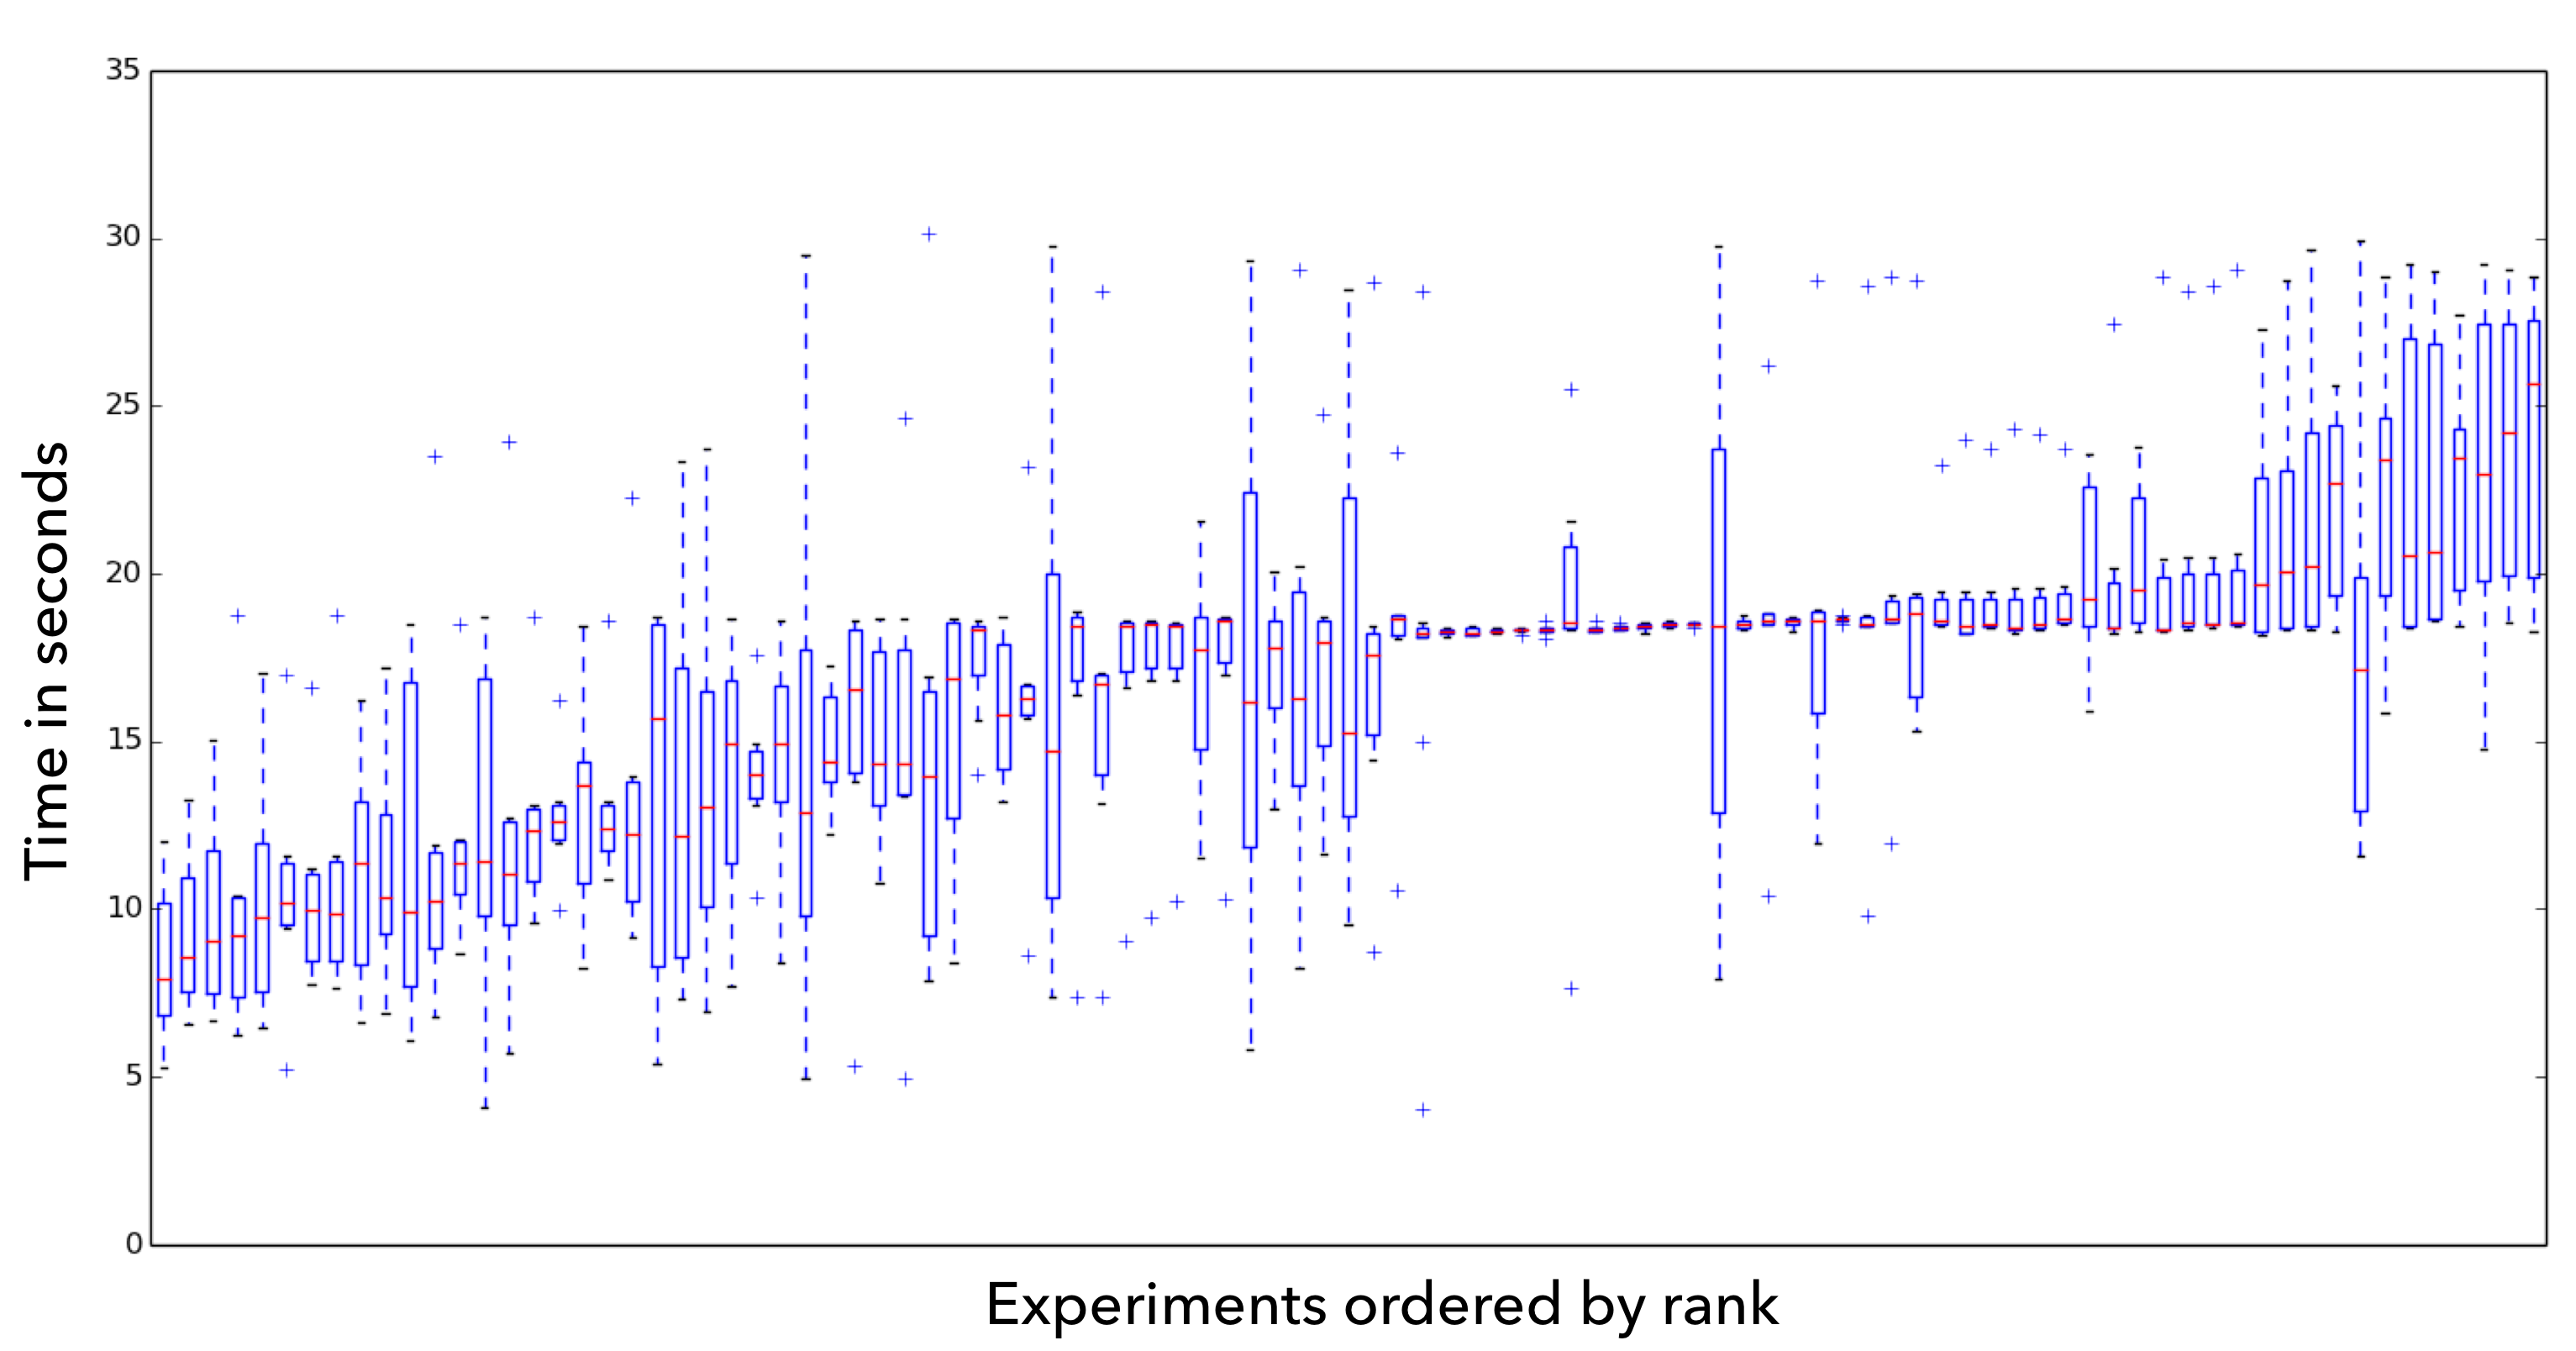
\includegraphics[width=3in]{img/2w_onemax_100_box.png}
    }
    \subfigure  [6 workers]
    {
        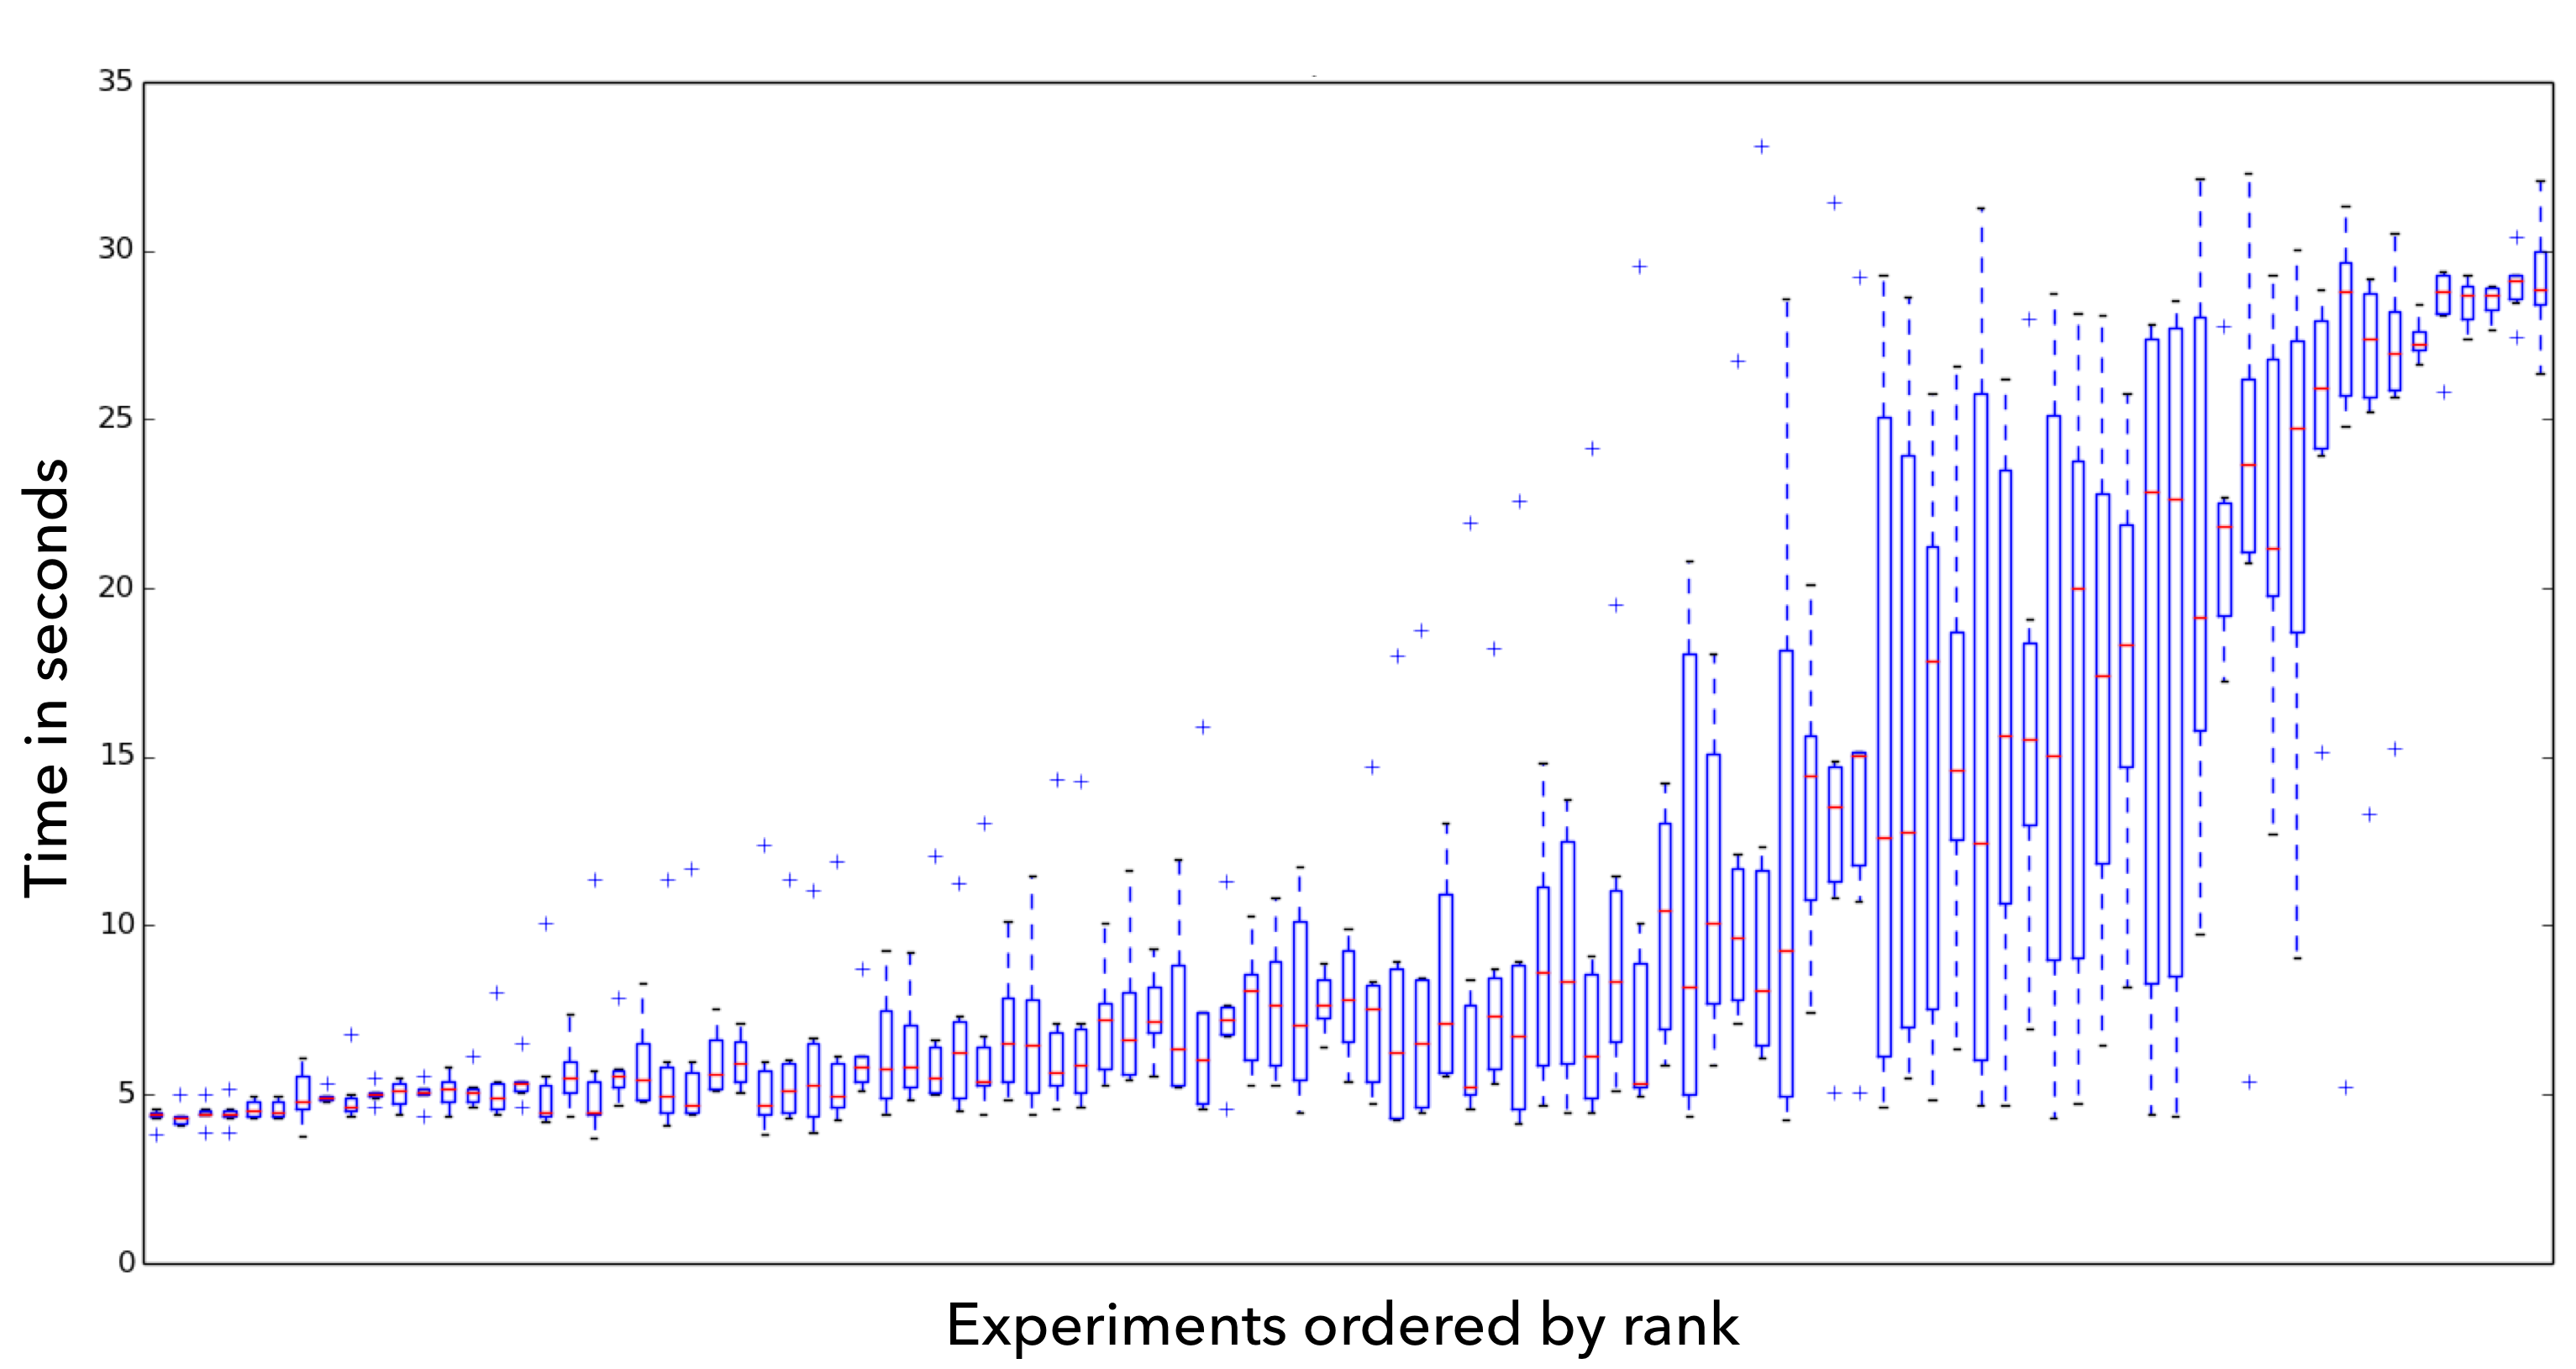
\includegraphics[width=3in]{img/6w_onemax_100_box.png}
    }
    \subfigure  [12 workers]
    {
        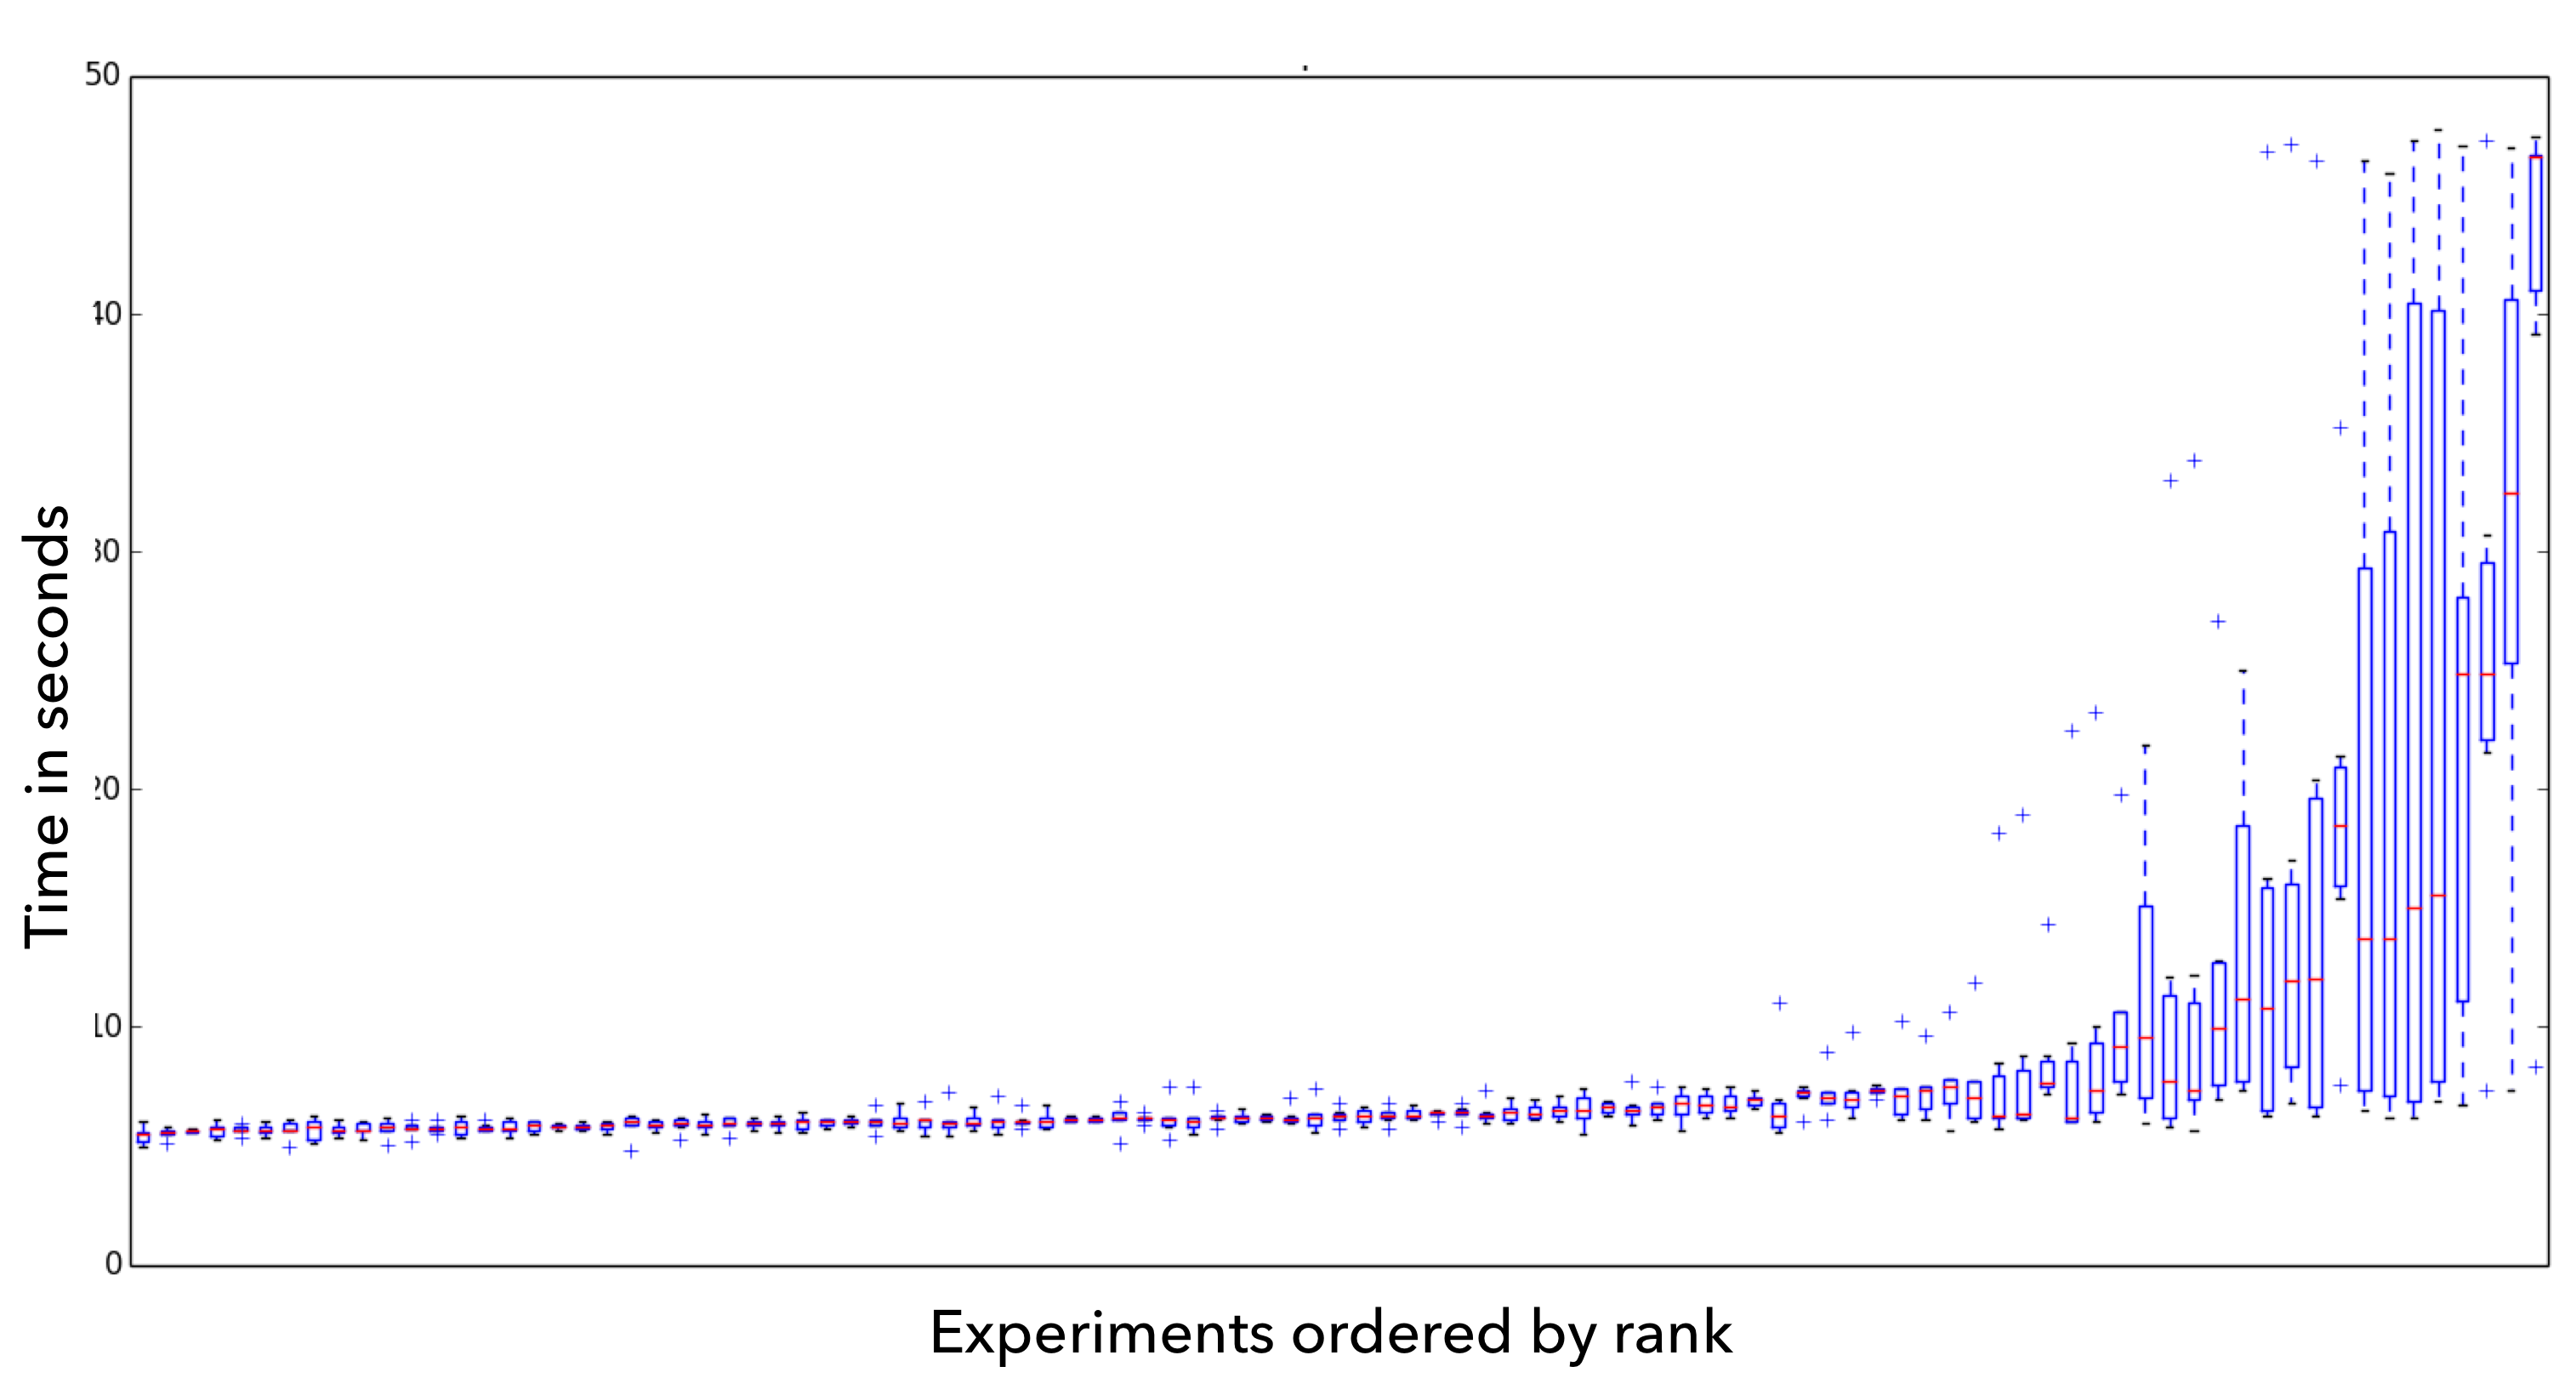
\includegraphics[width=3in]{img/12w_onemax_100_box.png}
    }

    \caption{100 experiments with random parameters for the 128 Bit OneMax problem.
    Experiments are ranked by the mean time to solution of 5 runs, with   
    (a) 2 workers, (b) 6 workers, and (c) 12 workers.}
    \label{fig:effort}
\end{figure*}


\begin{figure*}[t]
    \centering
        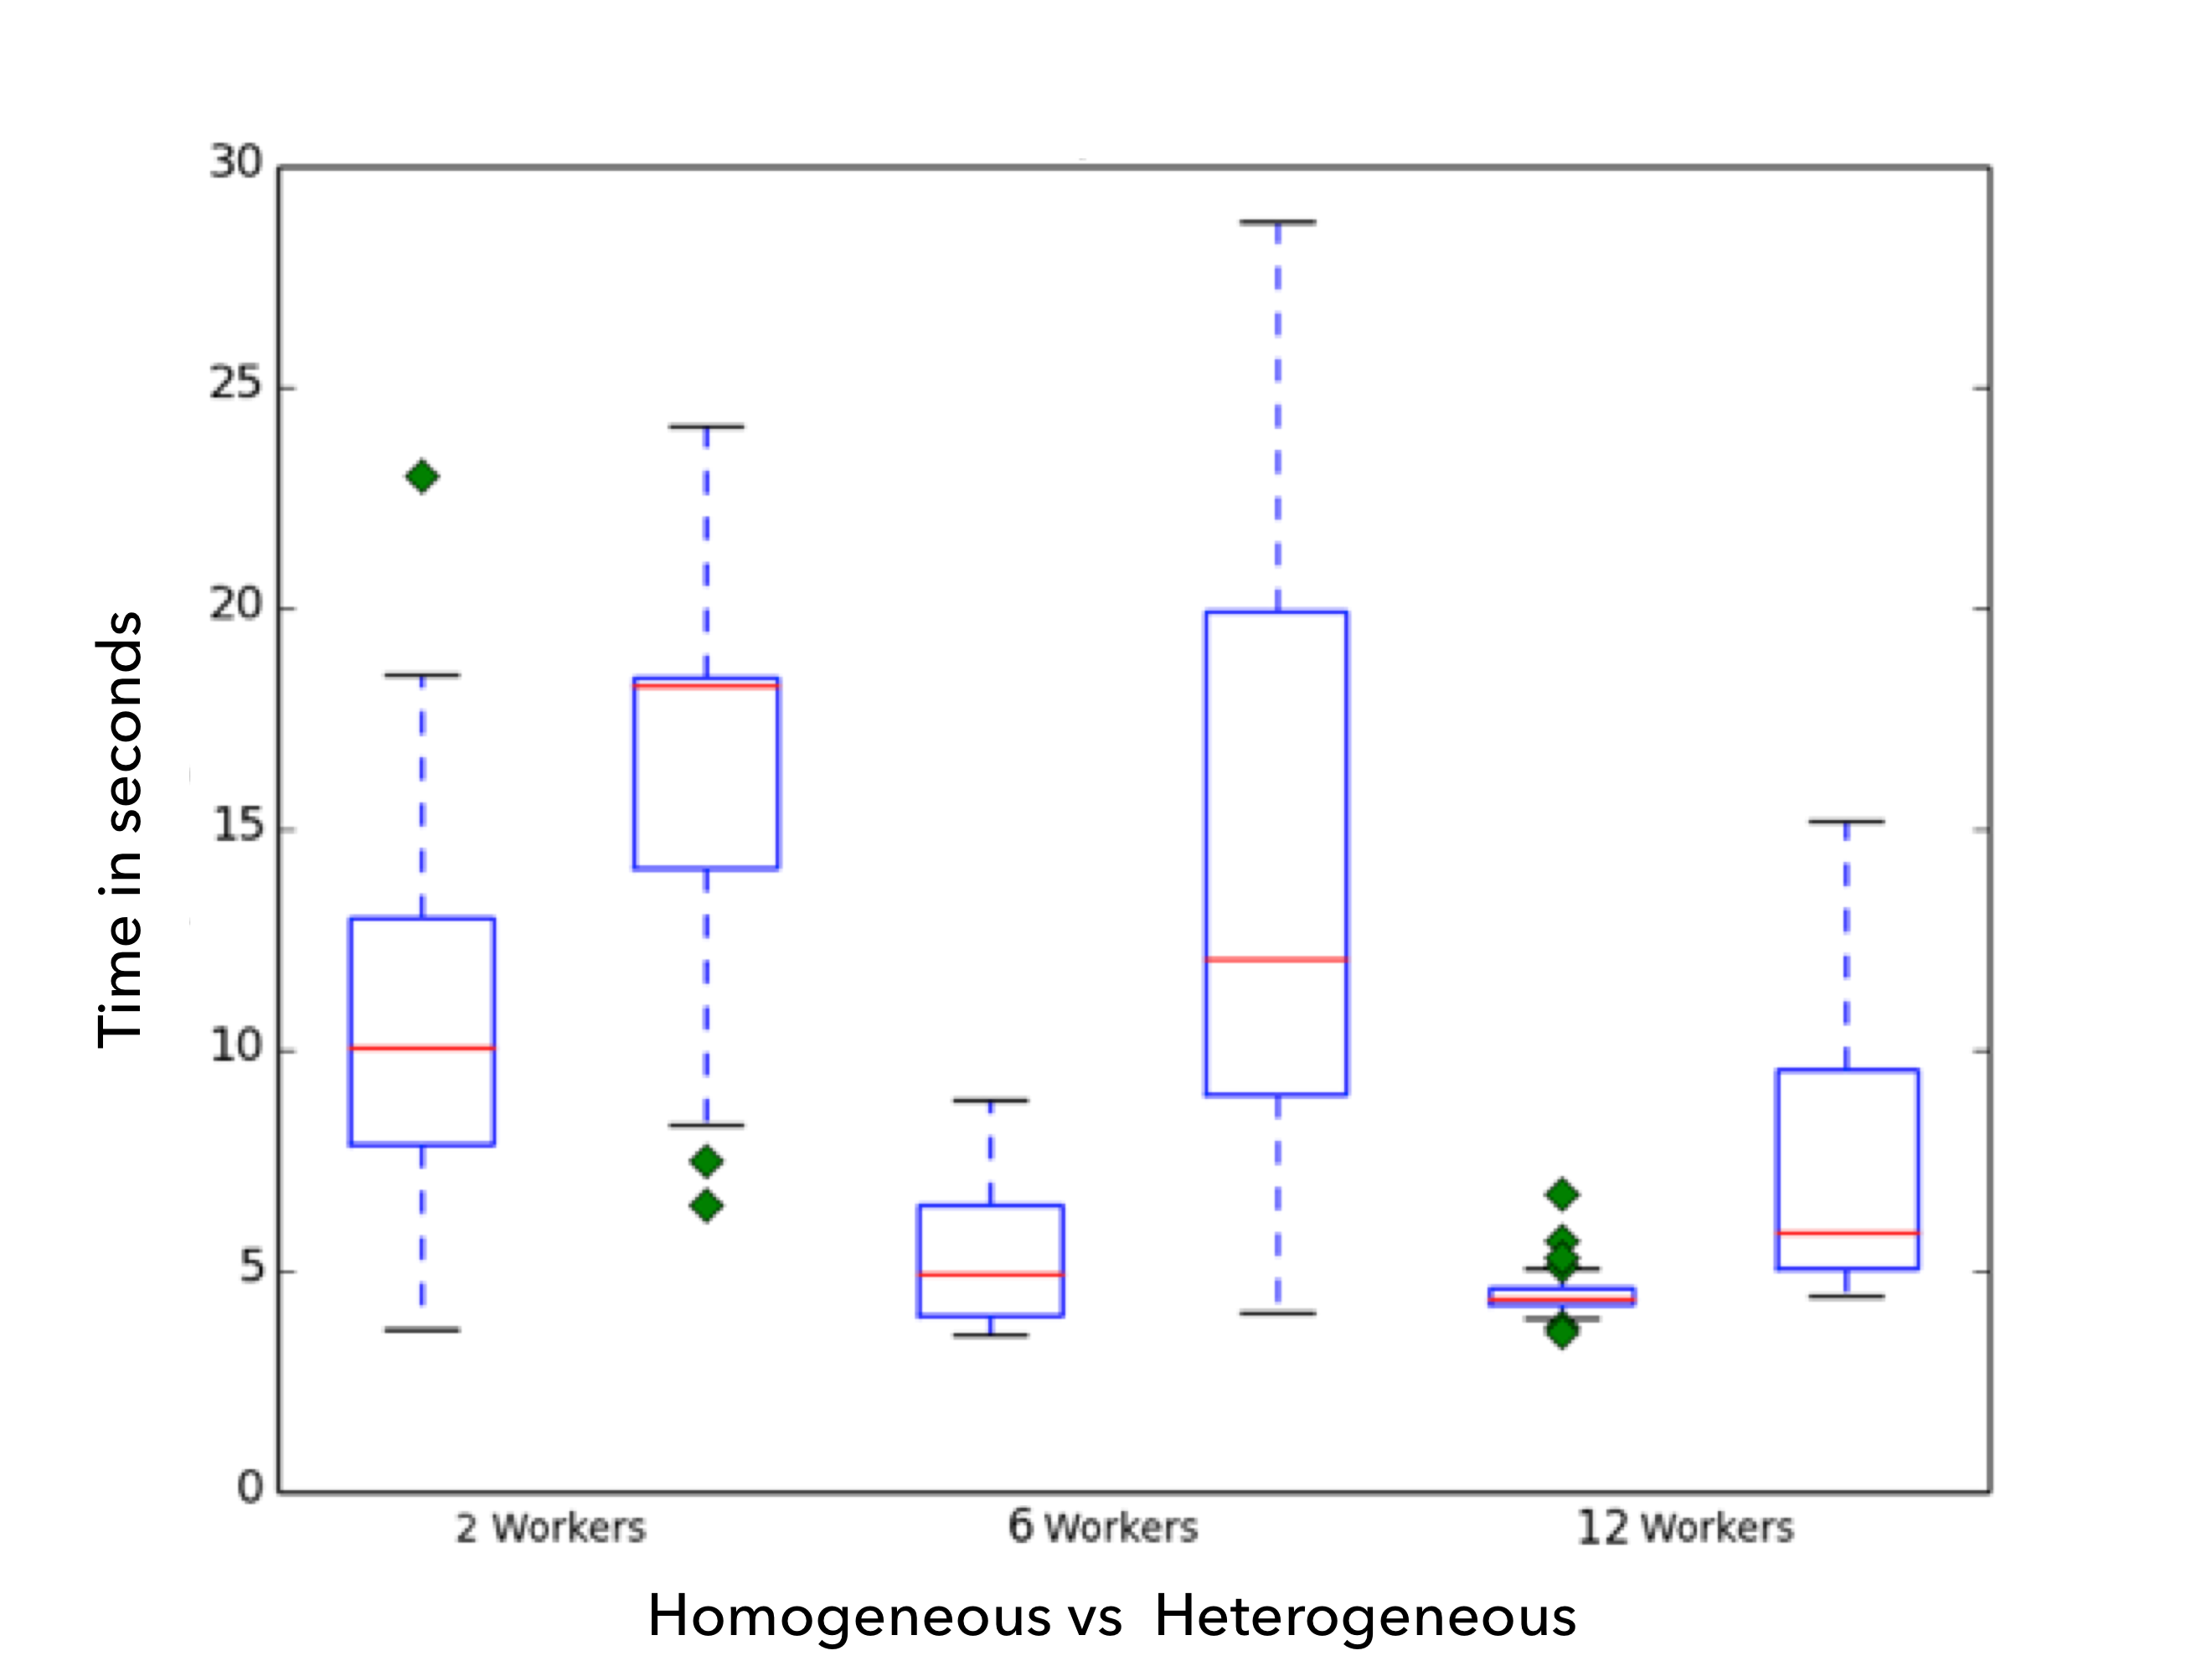
\includegraphics[width=10cm]{img/one_max_comp.png}
    \caption{Comparison of 30 runs of the 128 Bit OneMax problem. 
    Box-plot of the number of evaluations needed for solution, with a 2, 6 and 12 workers
    homogeneous configuration on the left side, and Heterogeneous configuration on the
    right side of each.
    }
    \label{fig:comp-onemax}
\end{figure*}


\subsection{ Single-Objective Optimization Test Functions}

\begin{figure*}[b]
    \centering
    \subfigure  [6 workers]
    {
        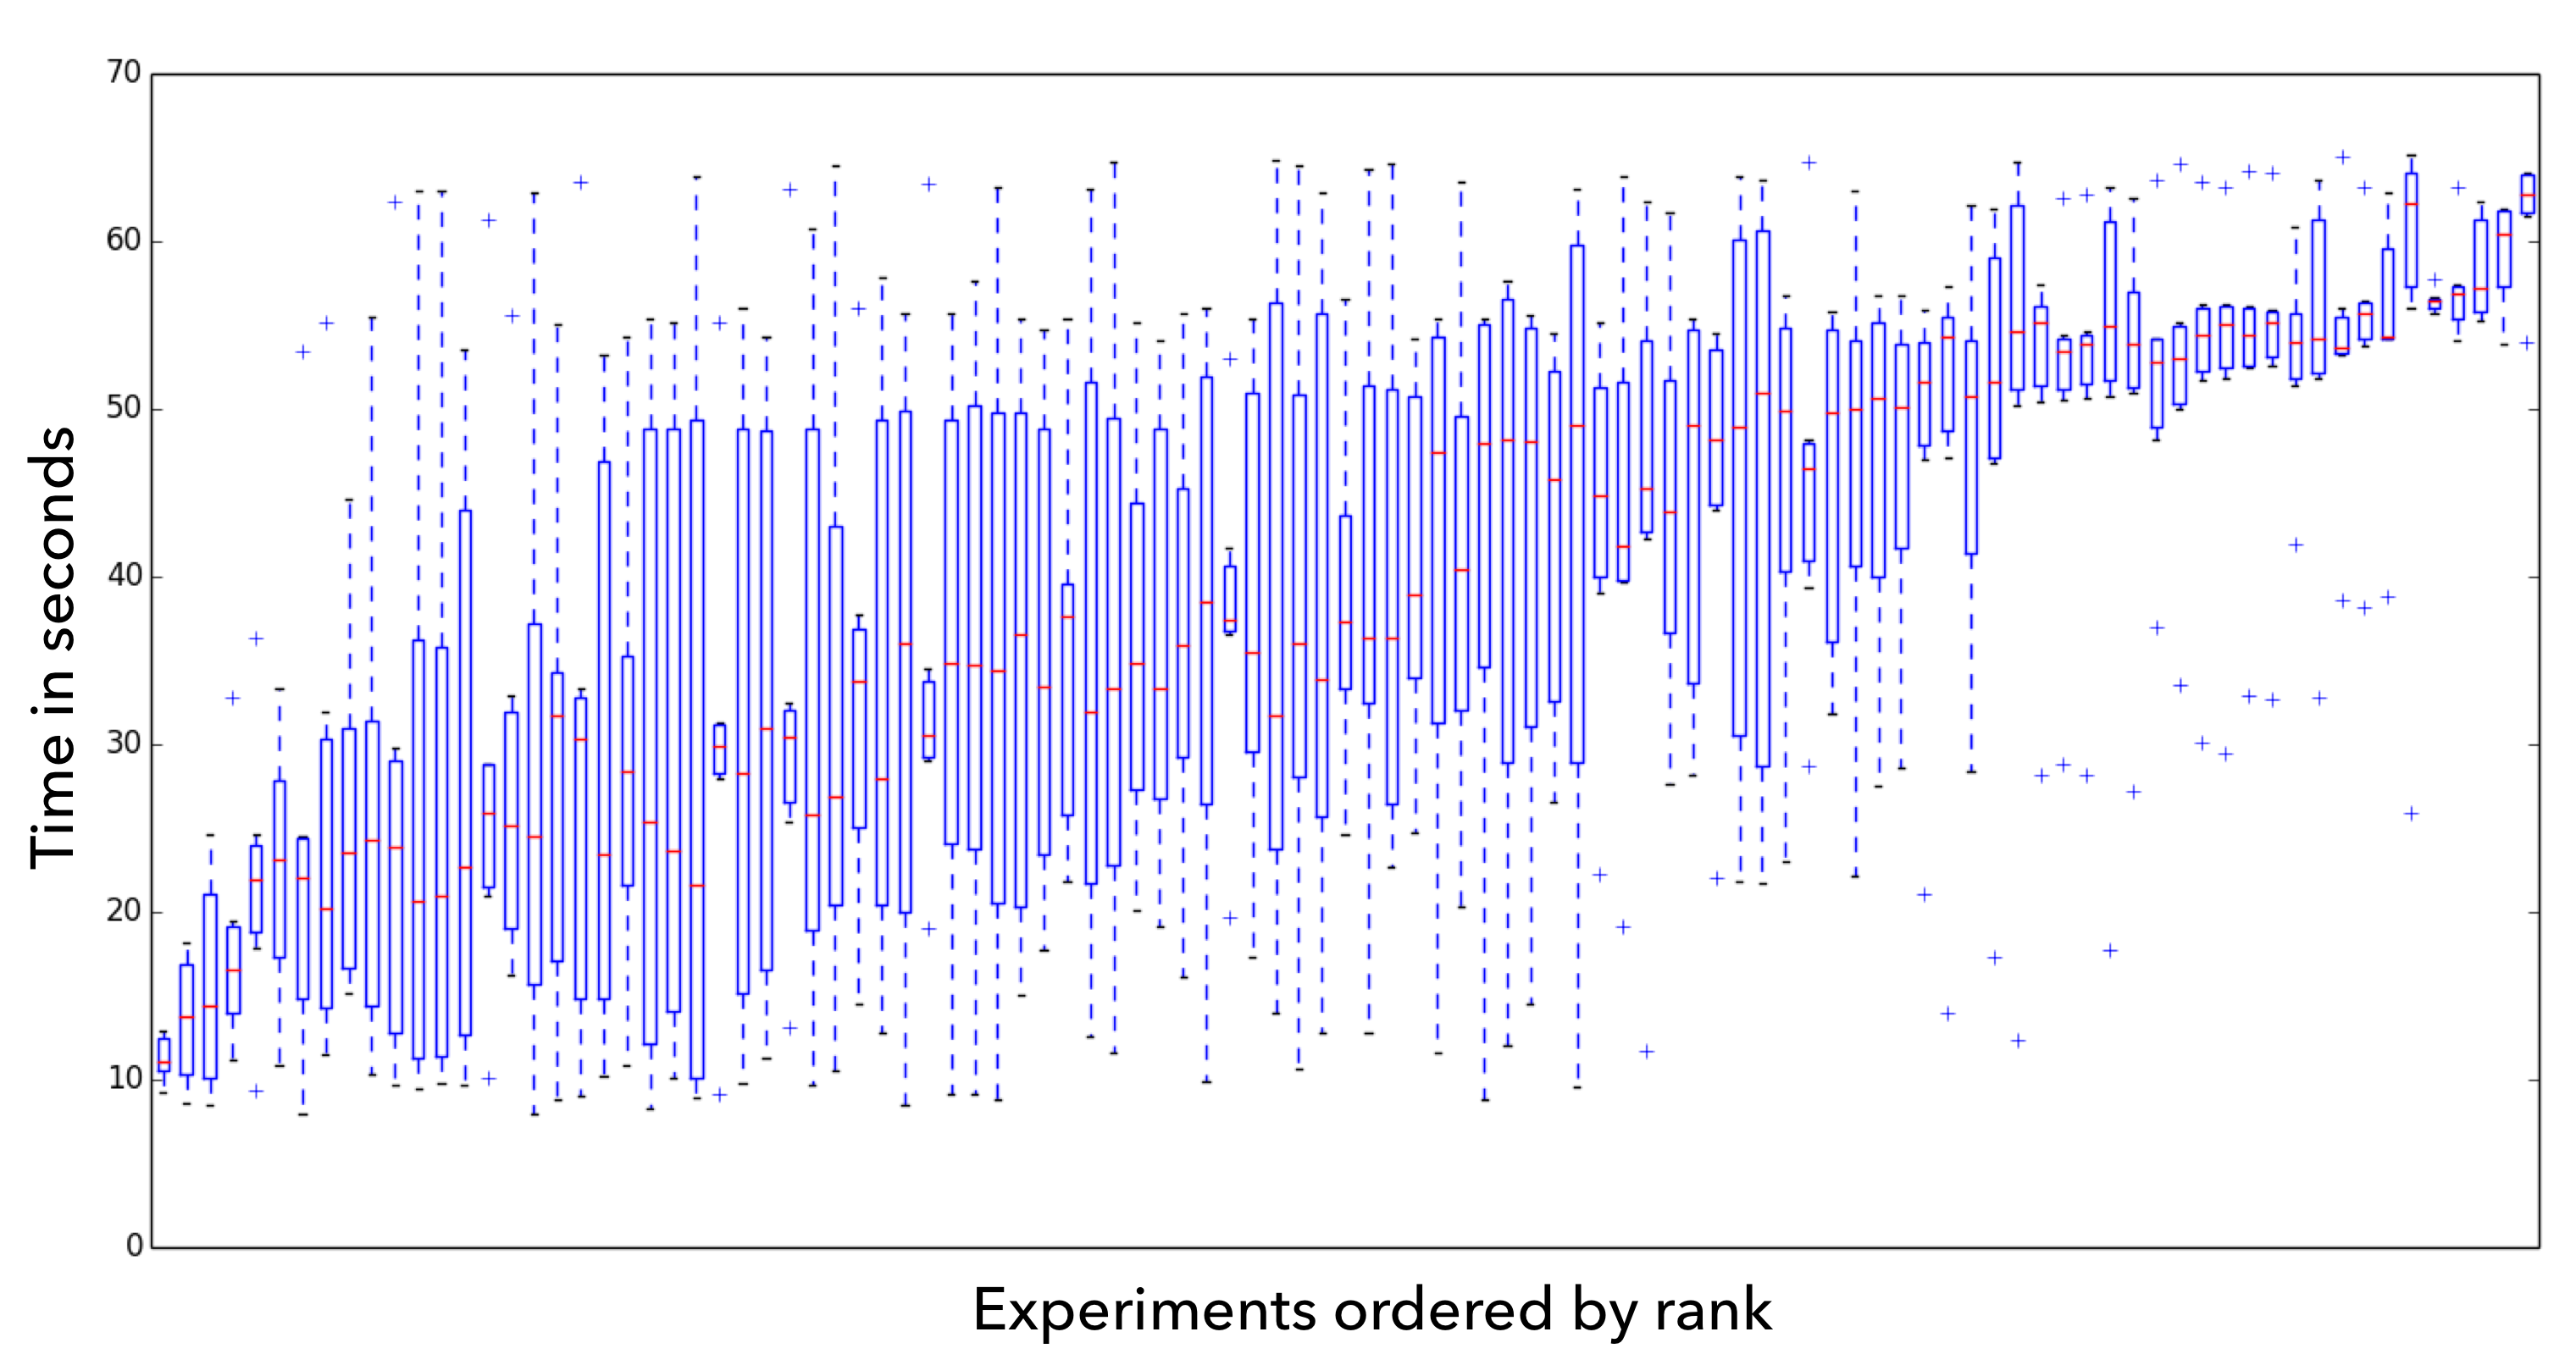
\includegraphics[width=2.2in]{img/6w_griewank_100_box.png}
    }
    \subfigure  [12 workers]
    {
        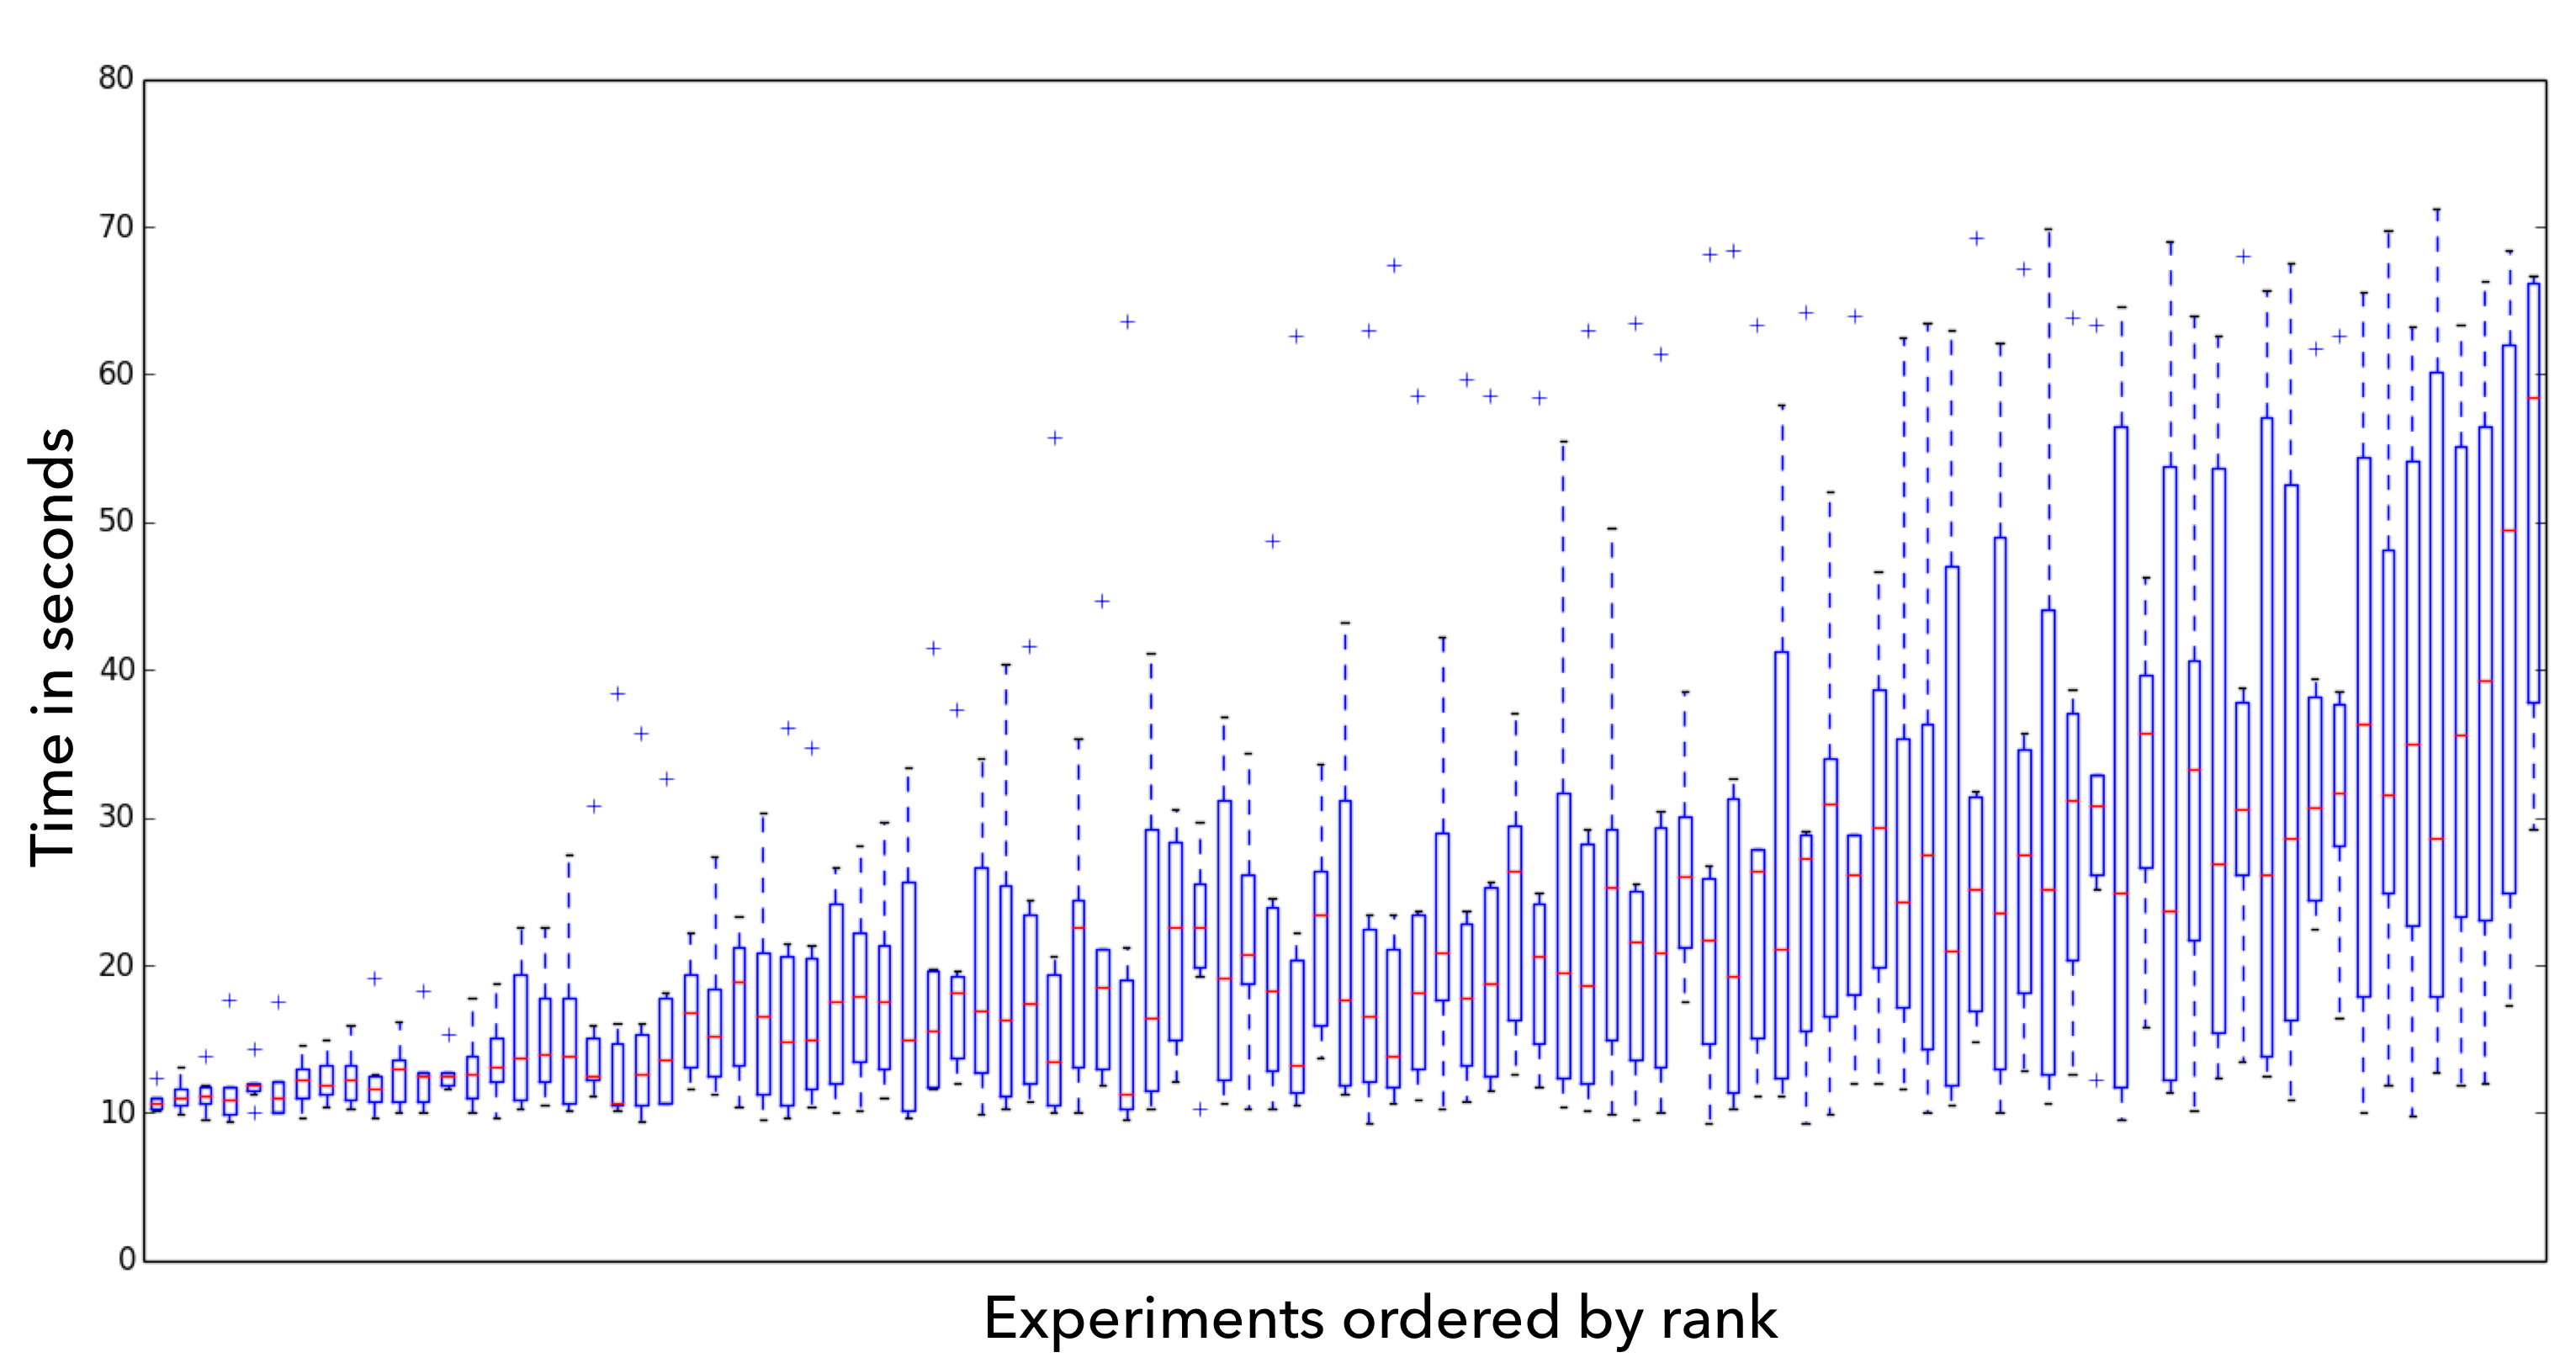
\includegraphics[width=2.2in]{img/12w_griewank_100_box.png}
    }

    \caption{100 experiments with random parameters for the 128 Bit Griewank 
    single-objective optimization test function. Experiments are ranked by 
    the mean time to solution of 5 runs, with (a) 6 workers, and (b) 12 workers.}
    \label{fig:griewank-homo}
\end{figure*}


\begin{figure*}[b]
    \centering
    \subfigure  [Homogeneous]
    {
        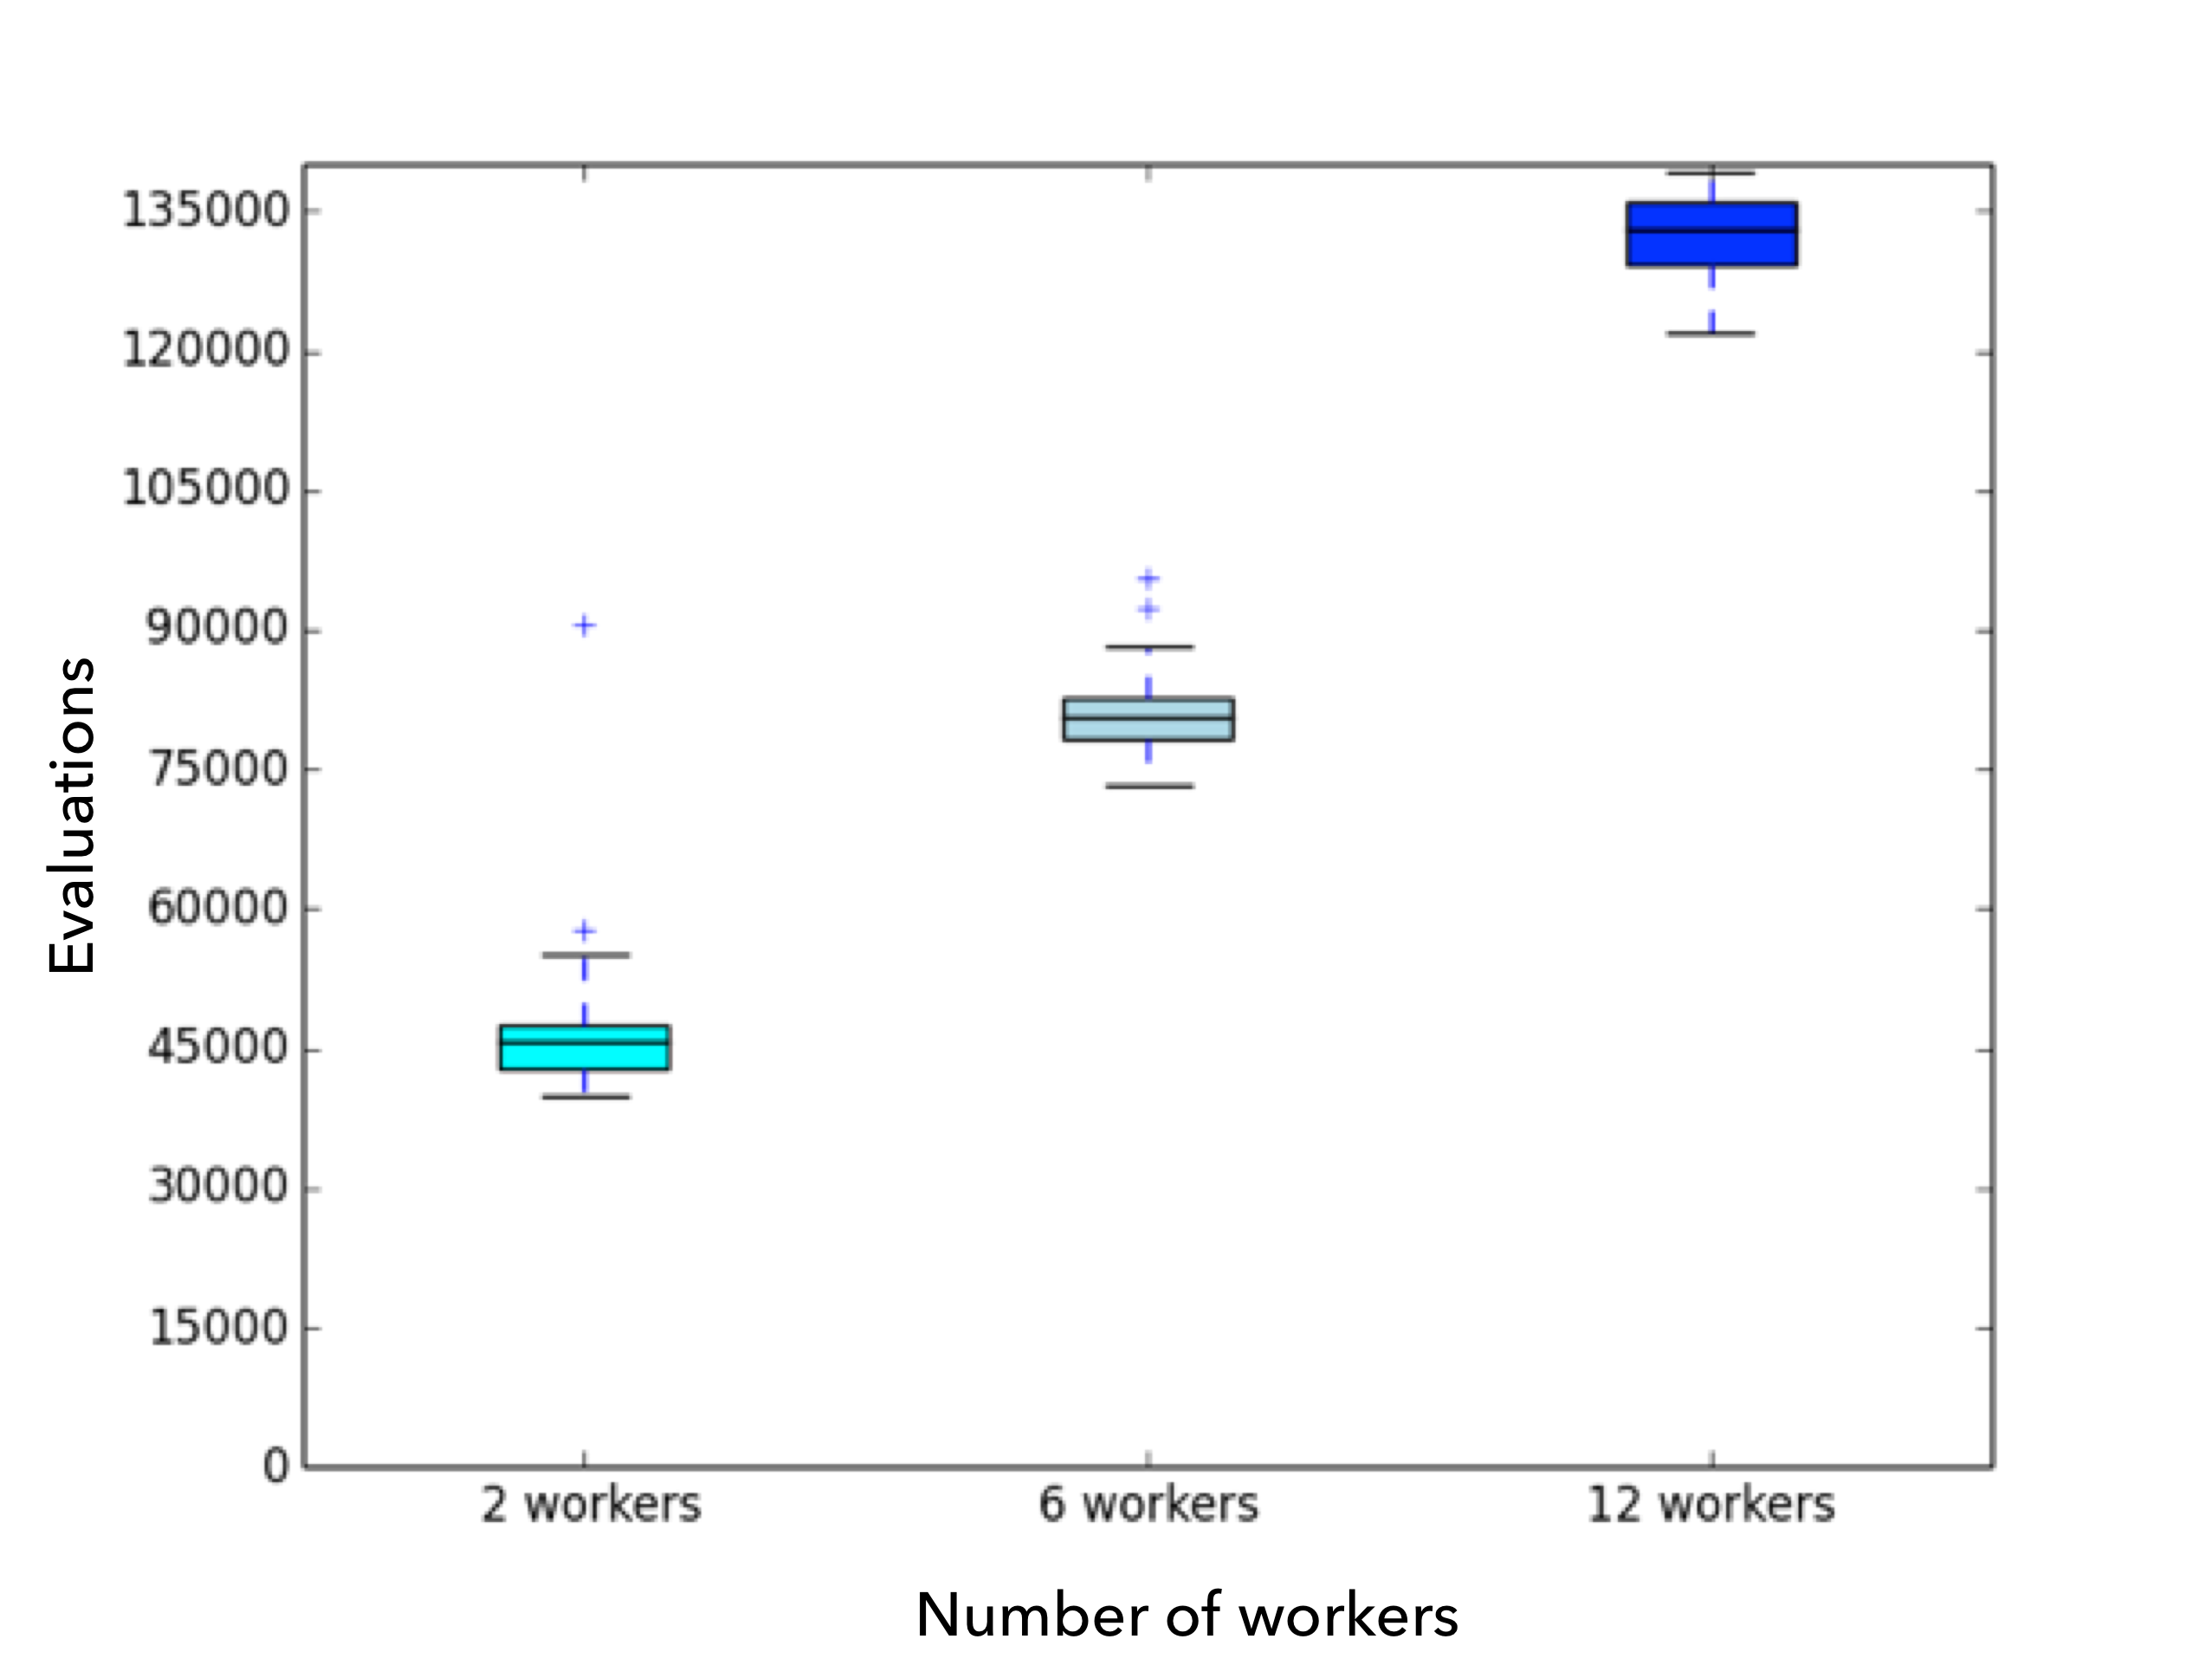
\includegraphics[width=2.2in]{img/griewank_evals_homo.png}
    }
    \subfigure  [Heterogeneous]
    {
        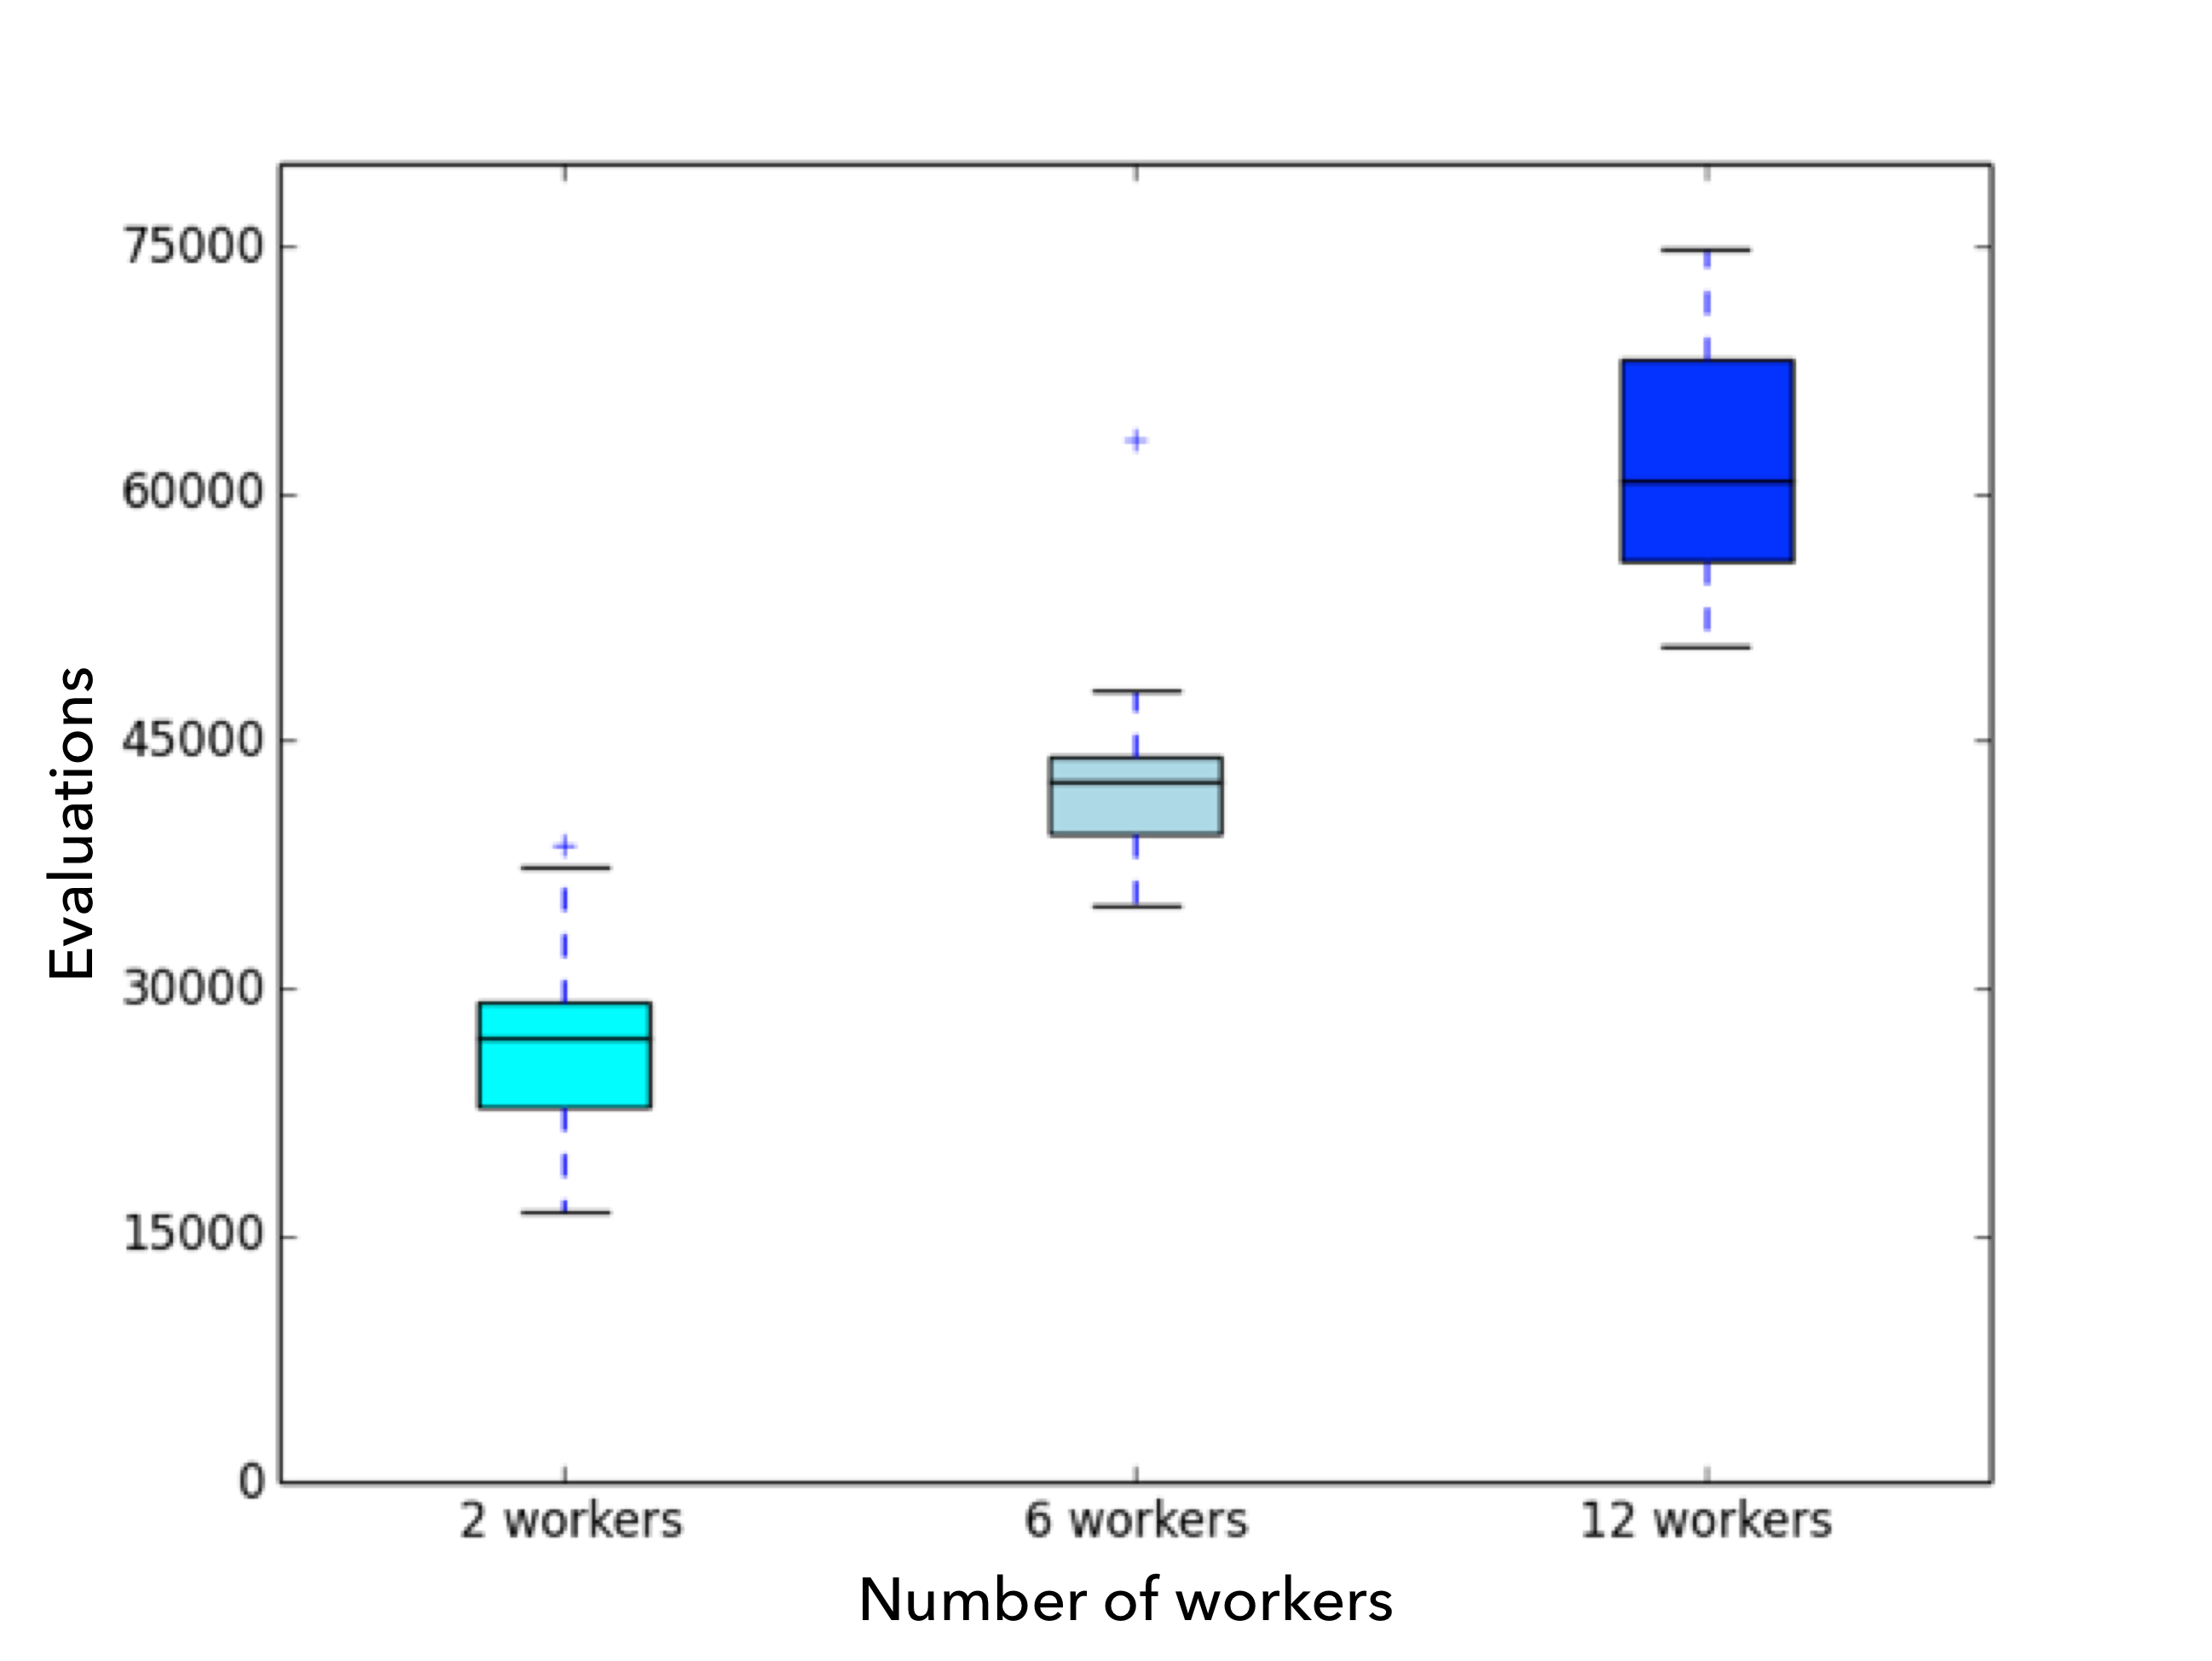
\includegraphics[width=2.2in]{img/griewank_evals_hetereo.png}
    }
      \caption{30 runs of the 128 dimension Griewank single-objective optimization test function. 
    Box-plot of the number of evaluations needed for solution, with an (a) Homogeneous configuration, and (b) Heterogeneous configuration.}
    \label{fig:griewank-evals}
\end{figure*}

\begin{figure*}[b]
    \centering
    \subfigure  [Homogeneous]
    {
        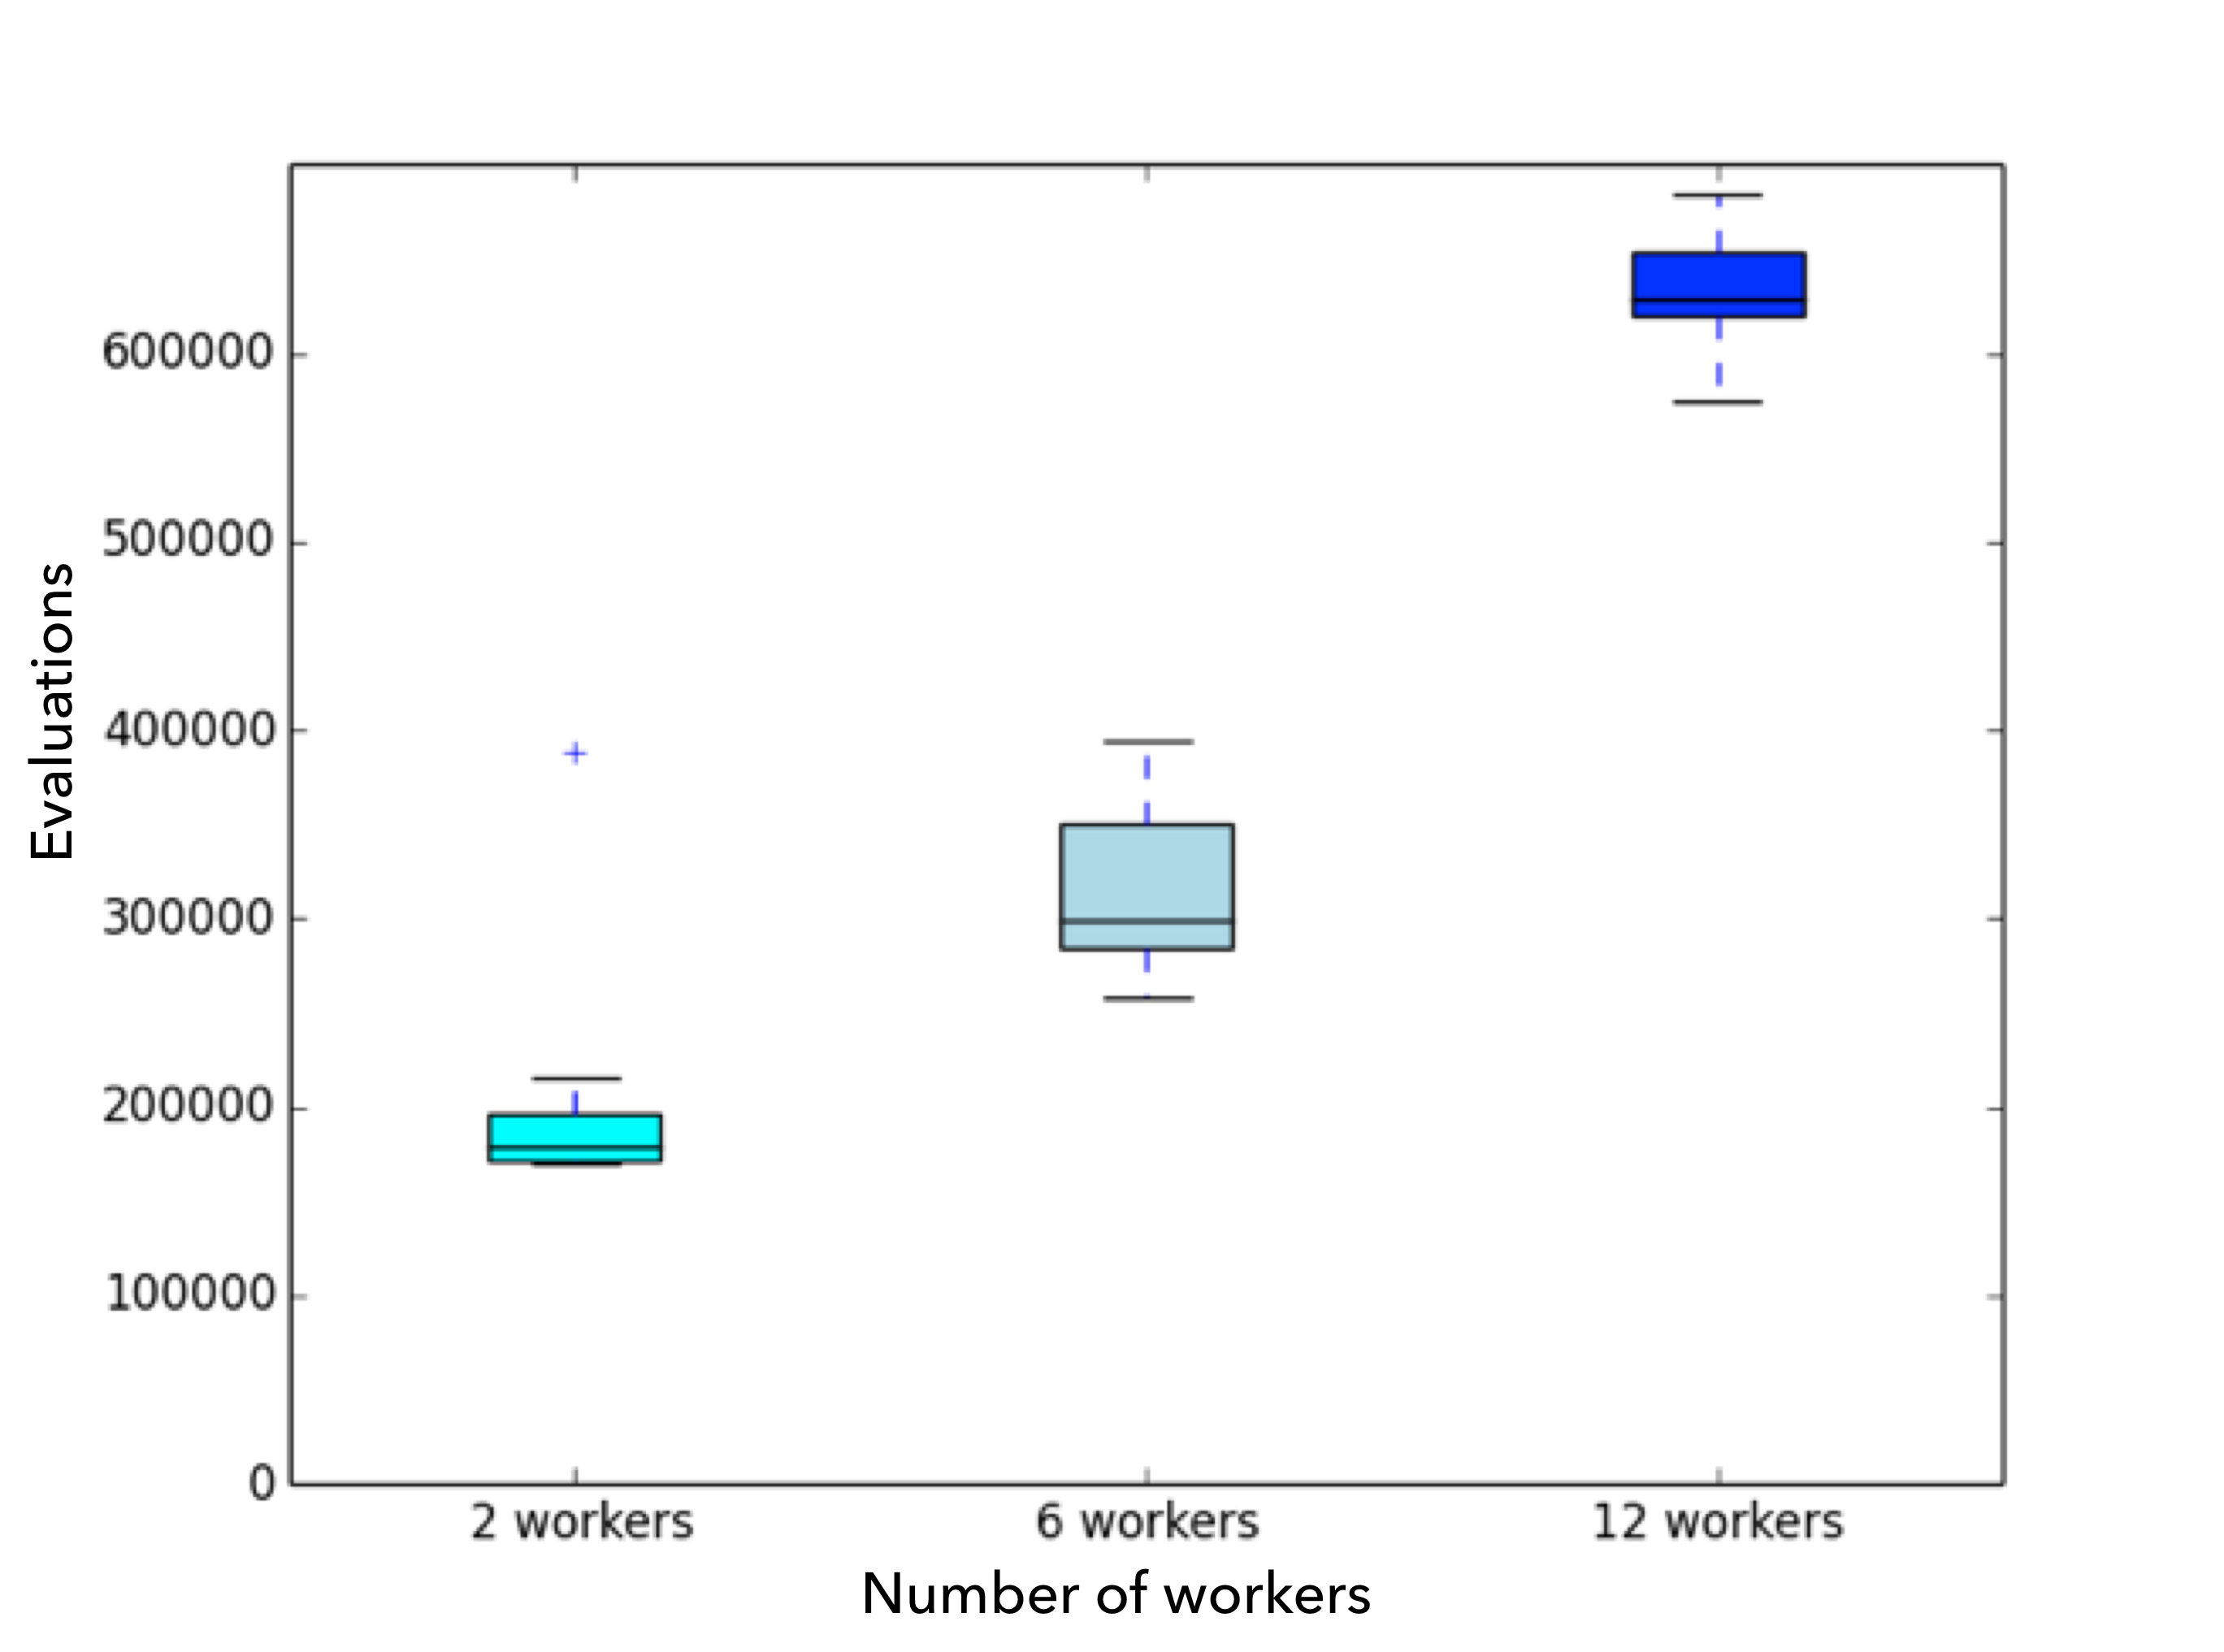
\includegraphics[width=2.2in]{img/schaffer_evals_homo.png}
    }
    \subfigure  [Heterogeneous]
    {
        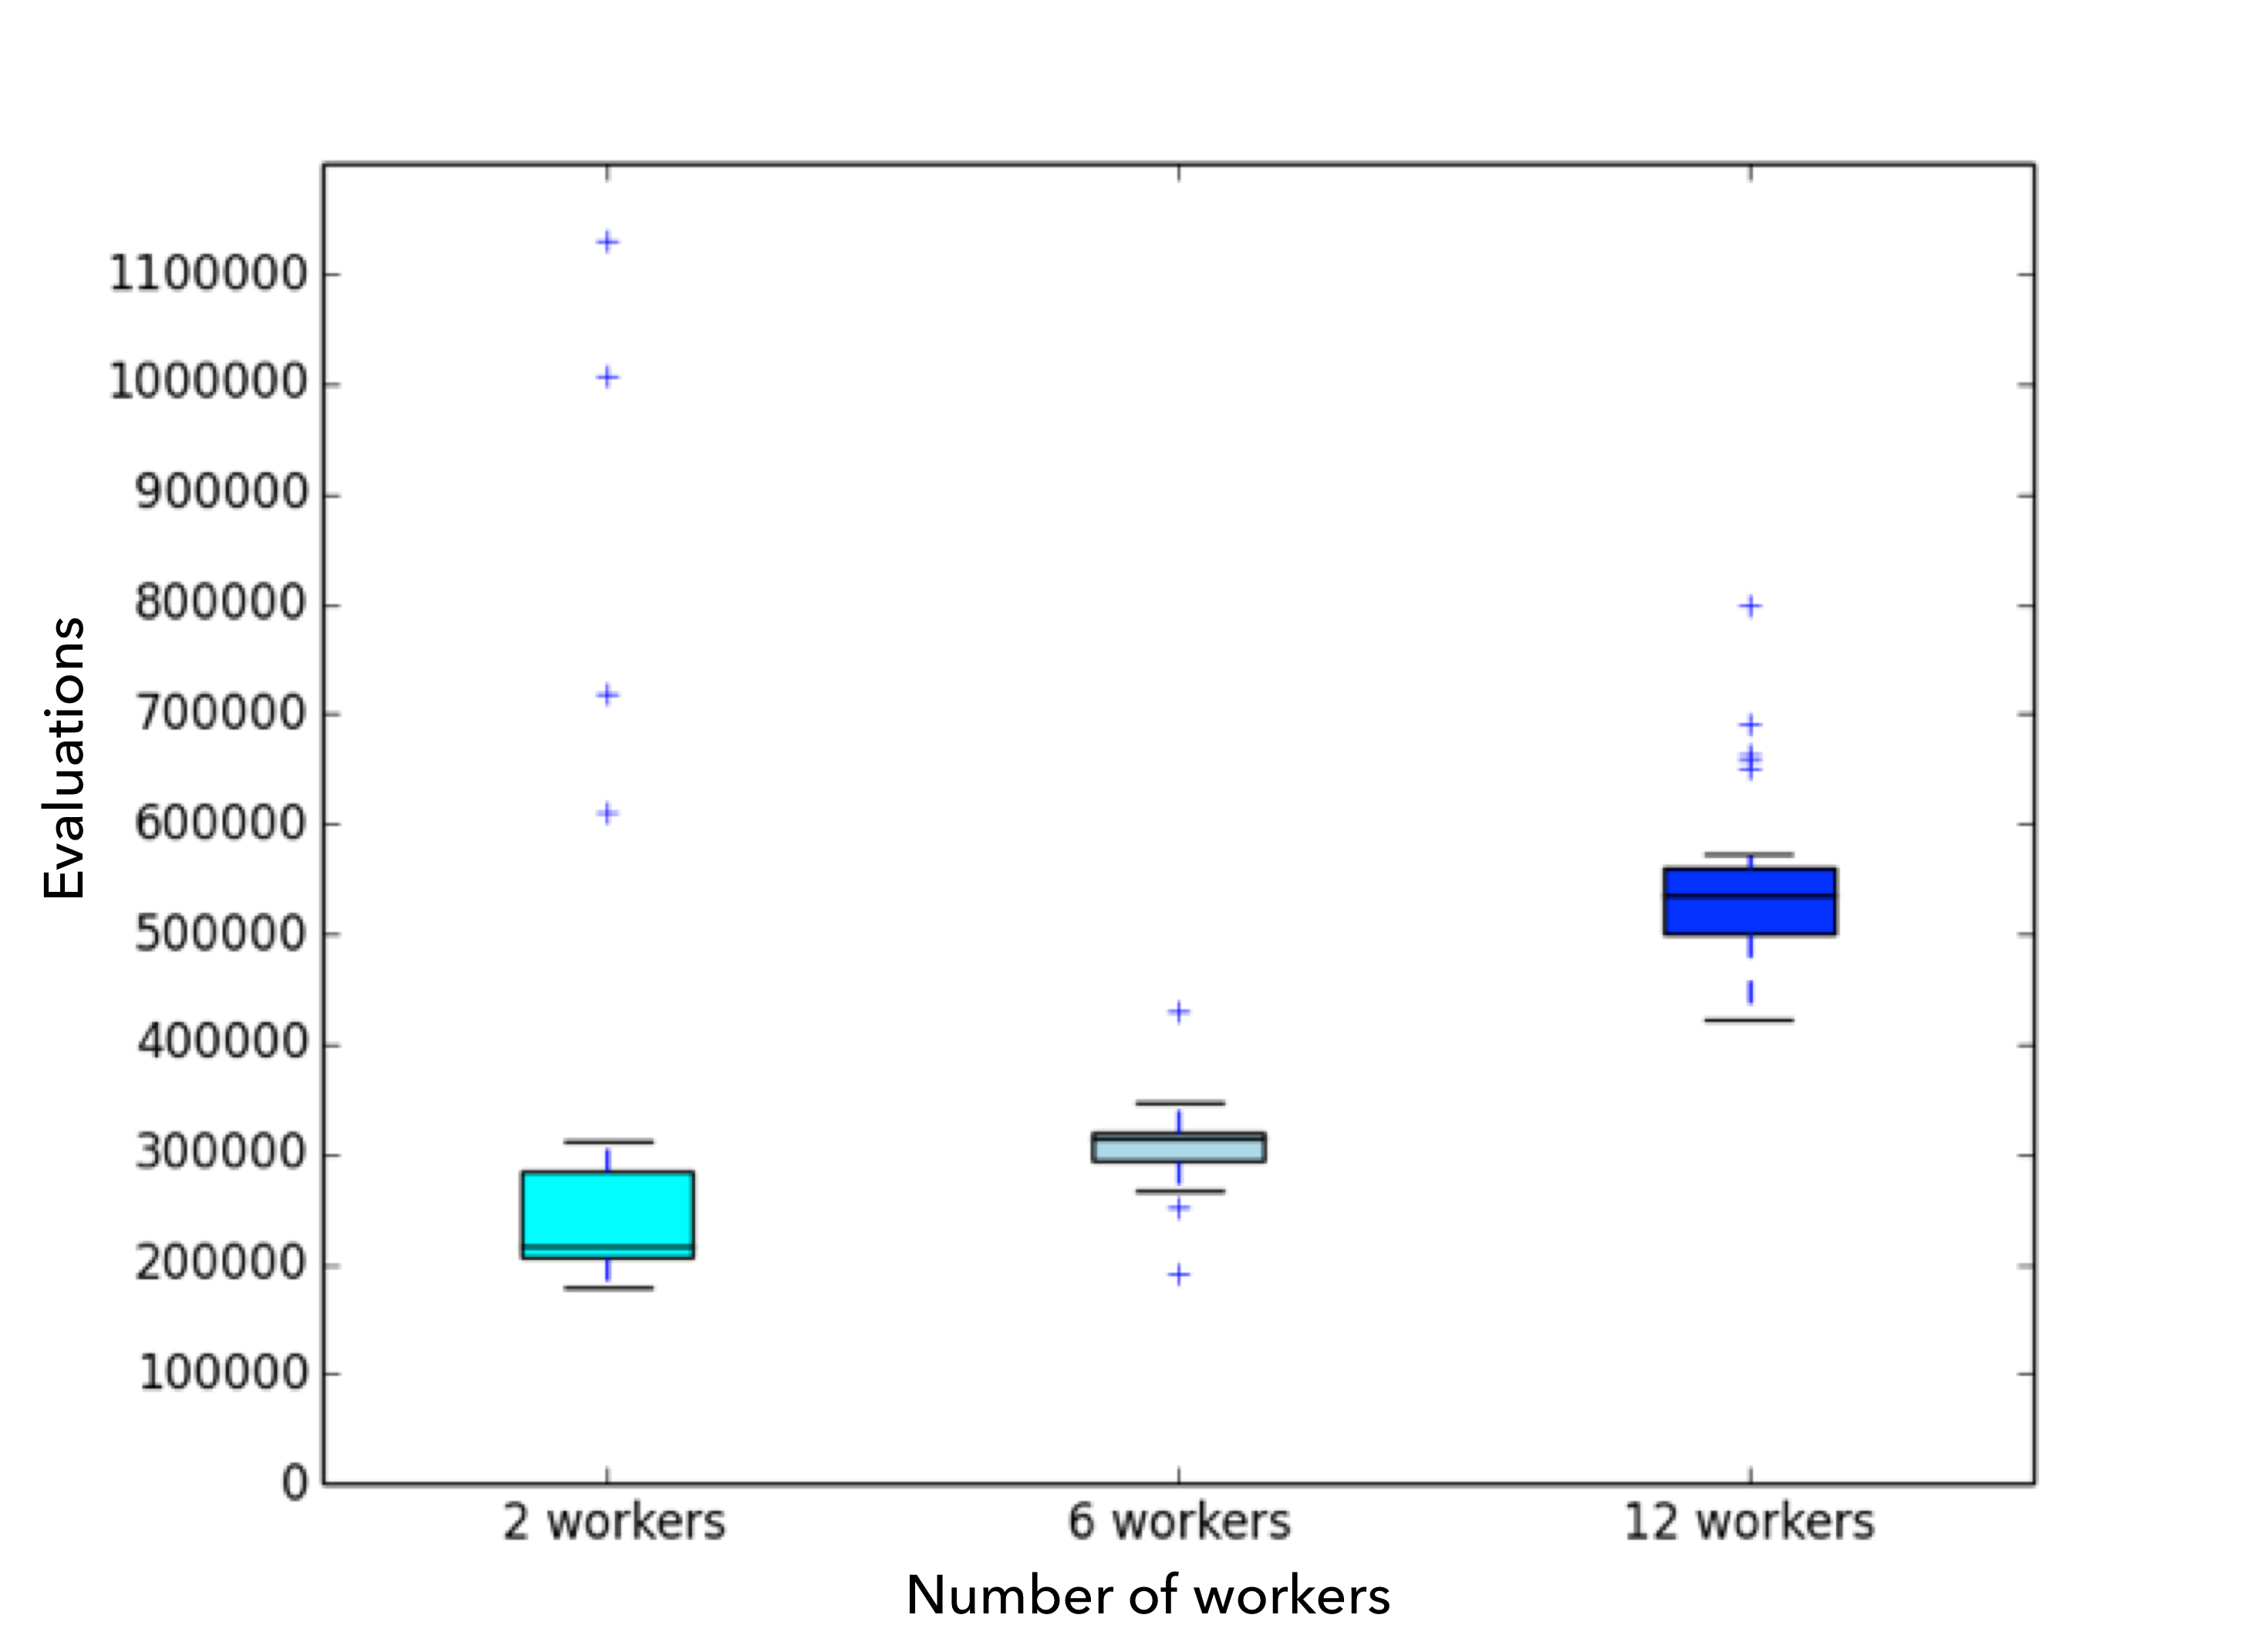
\includegraphics[width=2.2in]{img/schaffer_evals_hetereo.png}
    }
 

    \caption{30 runs of the 128 dimension Schaffer single-objective optimization test function. 
    Box-plot of the number of evaluations needed for solution, with an (a) Homogeneous configuration, and (b) Heterogeneous configuration.}
    \label{fig:schaffer-evals}
\end{figure*}

\begin{figure*}[t]
    \centering
        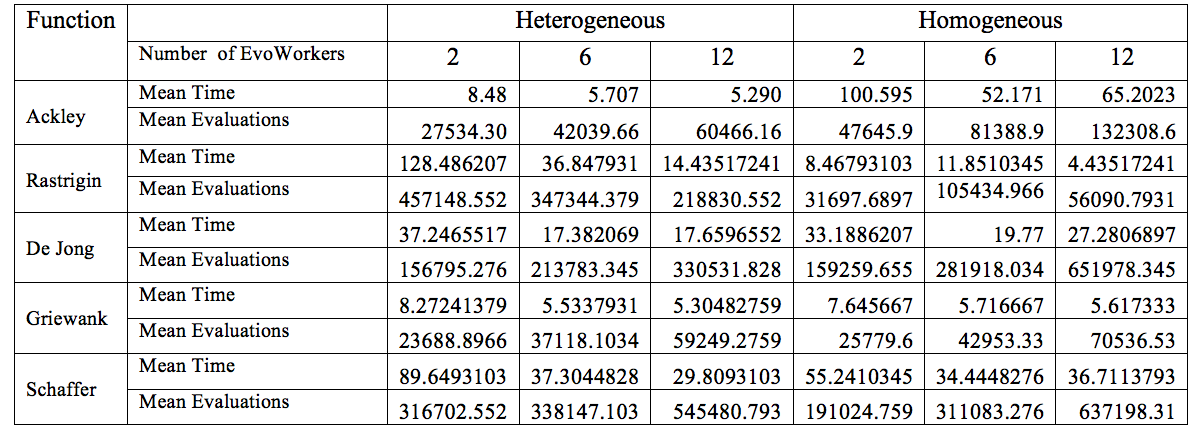
\includegraphics[width=10cm]{img/table.png}
    \caption{Summary table of results. }
    \label{fig:summary}
\end{figure*}

\end{document}
